\documentclass[11pt]{article}
\usepackage[small]{caption}
\usepackage{geometry}               
\usepackage{graphicx,epsfig,color}
\usepackage{hyperref}
%\DeclareGraphicsRule{.tif}{png}{.png}{`convert #1 `dirname #1`/`basename #1 .tif`.png}

% need to epstopdf figures first
\newif\ifpdf\ifx\pdfoutput\undefined\pdffalse\else\pdfoutput=1\pdftrue\fi
\newcommand{\pdfgraphics}{\ifpdf\DeclareGraphicsExtensions{.pdf,.jpg}\fi}
%

\captionsetup{width=1.07\textwidth}  
\usepackage{anysize}
\marginsize{1.5cm}{1.5cm}{1cm}{2cm}

\usepackage{textcomp}

\date{}                                          

\begin{document}

\title{\bf{T2K GRID processing}}

\author{{\slshape J. Perkin$^a$, B. Still$^b$, G. Wikstr\"{o}m$^c$$^*$}\\[1ex]
$^a$University of Sheffield, Sheffield, United Kingdom\\
$^b$Queen Mary University of London, London, United Kingdom\\
$^c$DPNC, Universit\'{e} de Gen\`{e}ve, Geneva, Switzerland\\
$^*$No longer an active T2K collaborator}

\maketitle

\abstract{
\noindent This technical note contains documentation regarding the
GRID processing for the T2K experiment. The general structure of the
GRID and the related T2K software \verb+nd280Computing+ is described and a
detailed user's manual for the interface scripts is given. We also
present some benchmark performance numbers.
}


\vspace{10cm} 
T2K-TN-049

\thispagestyle{empty}

\newpage

\tableofcontents

\newpage

%%%%%%%%%%%%%%%%%%%%%%%%%%%%%%%%%%%%%%%%%%%%%%%%%%%%%%%%%%%%%%%%%%%%%%%%%%
\section{Introduction}
%%%%%%%%%%%%%%%%%%%%%%%%%%%%%%%%%%%%%%%%%%%%%%%%%%%%%%%%%%%%%%%%%%%%%%%%%%
\label{sec:intro}

The T2K experiment uses the GRID computing extensively to process
ND280 data and Monte Carlo (MC). 

\subsection{The GRID}
The GRID consists of a set of computing elements (CEs) and storage
elements (SEs) connected through workload management servers (WMSs)
and central databases. Through the \verb+gLite+ interface a user can
submit a job to a central system without having to worry about the
location of the resources (data and CPU) and moreover store the output
directly on the GRID.

What is referred to as the GRID here, is a part of the Worldwide LHC
Computing GRID (wLCG) \cite{lcg}, which has been developed for the LHC
experiment at CERN. T2K currently uses mainly sites connected to the
UK GridPP network \cite{gridpp}, with additional sites across Eurpoe.
Together with Westgrid in Canada, it performs the main computing tasks
for T2K.

The general structure of the GRID is described schematically in
Fig.~\ref{fig:schematic}.

\begin{figure}[!h]
  \begin{center}
    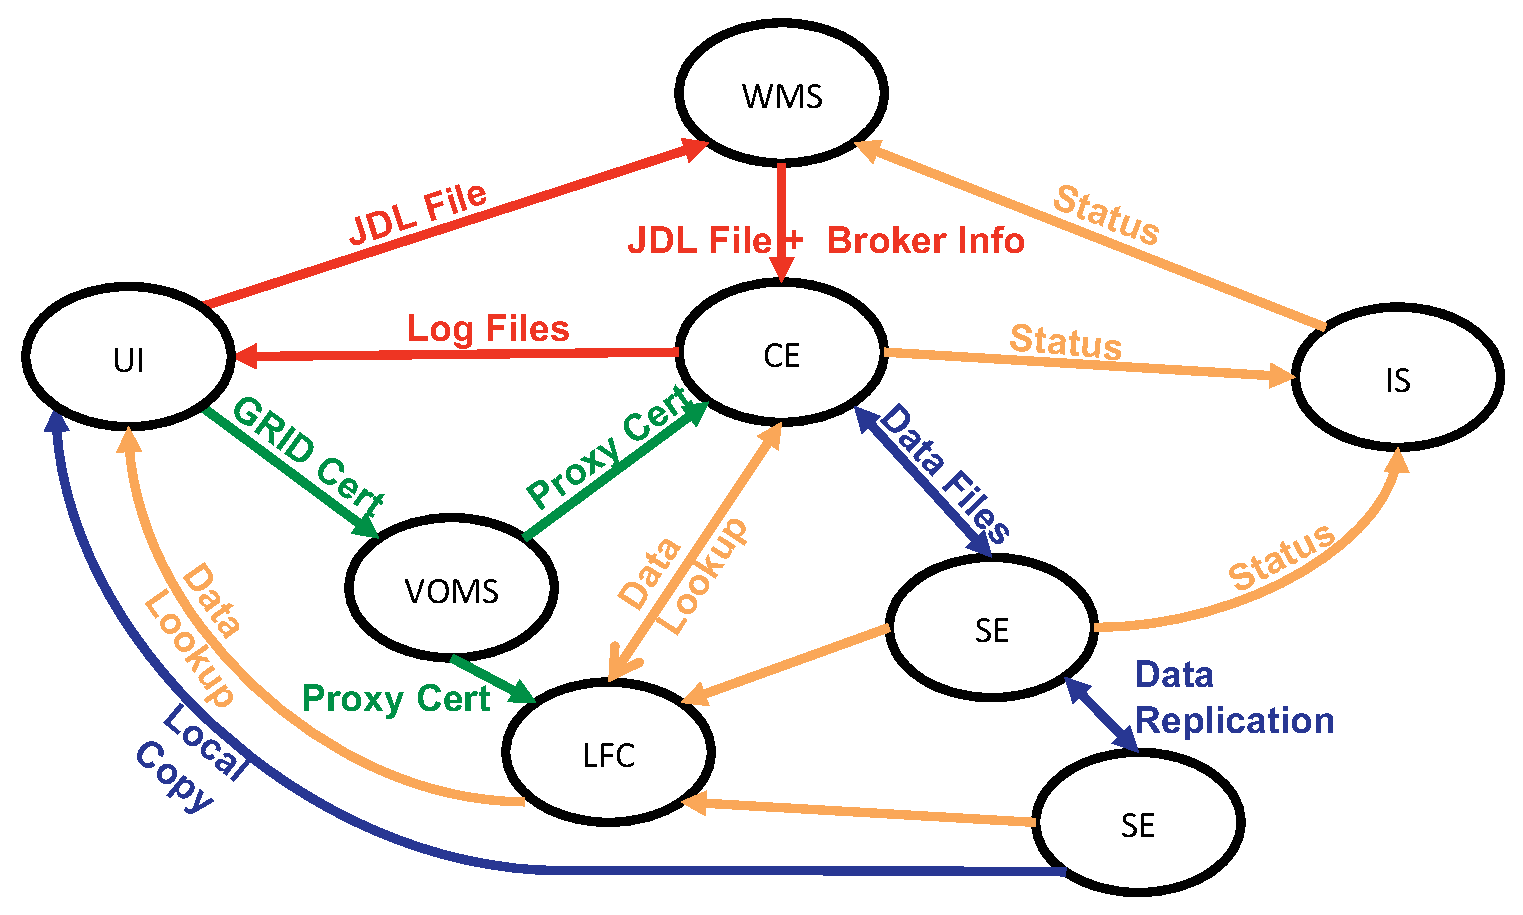
\includegraphics[width=0.7\textwidth]{gridoverview}
    \caption{\label{fig:schematic} A schematic overview of how the GRID works, explained in the text.}
  \end{center}
\end{figure}

\subsubsection*{Certificate}
Every GRID user needs a GRID certificate acting as a digital ID
card. This can be obtained from the local Certificate Authority
(CA), usually at the user's institution. A certificate is personal and
is in general valid for one year.

\subsubsection*{Virtual Organisation}
On the GRID, it is the virtual organisation (VO) \cite{cic}, not the
individual user, that runs the job. The VO for T2K is
\verb+t2k.org+. A user can join a VO with his/her certificate. The
authentication information is handled by a Vitual Organisation
Managements Server (VOMS).


\subsubsection*{\texttt{gLite}}
The interface between a user and the GRID, and within different
elements on the GRID, is done through the \verb+gLite+ \cite{glite},
GRID computing middleware. The end user interface is via \verb+gLite-UI+, which reads
the status of jobs from the information service (IS).

\subsubsection*{Computing elements}
The \verb+t2k.org+ VO currently processes data on the following
computing elements (CEs):
\begin{itemize}
\item RAL: \verb+lcgce05.gridpp.rl.ac.uk+
\item Imperial: \verb+ceprod03.grid.hep.ph.ic.ac.uk+,
  \verb+ceprod04.grid.hep.ph.ic.ac.uk+,\\
  \verb+ceprod05.grid.hep.ph.ic.ac.uk+,
  \verb+ceprod06.grid.hep.ph.ic.ac.uk+
\item Liverpool: \verb+hepgrid5.ph.liv.ac.uk+, \verb+hepgrid6.ph.liv.ac.uk+
\item Sheffield: \verb+lcgce0.shef.ac.uk+, \verb+lcgce1.shef.ac.uk+
\item QMUL: \verb+ce02.esc.qmul.ac.uk+, \verb+ce03.esc.qmul.ac.uk+,
  \verb+ce04.esc.qmul.ac.uk+
\item Barcelona: \verb+ce05.pic.es+, \verb+ce06.pic.es+, \verb+ce07.pic.es+, \verb+ce08.pic.es+.
\end{itemize}
Each CE is a cluster consisting of hundreds of computing nodes. In
addition to the UK sites listed above, other European sites are
becoming available to \verb+t2k.org+.

\subsubsection*{Storage elements}
Every CE is attached to a high capacity disk array, known as the
storage element (SE). On every SE \verb+t2k.org+ has an allocated
storage area with a limited space. Both the raw and processed data are
stored on the SE. In order to limit data transfer within the GRID it
is desirable to run jobs on a CE attached to the SE where the input
data is, and also to store the output data there. The address of files
on an SE is determined by the storage URL or SURL and is prefixed with
\verb+srm://+ indicating the storage resource manager (SRM) protocol.

\subsubsection*{WMS}
The role of the workload management servers (WMSs) is to monitor the
load on CEs and submit jobs to those with available processing
capacity. They also check that input data is available and that job
requirements, such as the availability of a specific software release,
are met for a certain CE. When a match is found the WMS transfers the job
to the CEs queue. The GRID user submits jobs directly to one or more WMSs.

\subsubsection*{LFC/LFN/GUID}
The LCG File Catalogue (LFC) is used by \verb+t2k.org+. A GRID file is
registered to the LFC with a logical file name (LFN) that is independent
of its physical location on an SE. Thus the LFC represents a
convenient interface for the user, that links to files under a simple
alias, such that the actual location doesn't have to be
known. Synonymous with the LFN is the GUID a unique GRID file
identifier. GUIDs are required for example when unregistering files
from the LFC. A file in the LFC can and usually will have several
replicas. The files for \verb+t2k.org+ are linked to \verb+lfn:/grid/t2k.org/+.

\subsubsection*{JDL}
The GRID jobs are specified in files written in job description language (JDL). It specifies input and output files, job executable and arguments, and general settings and requirements.

\subsubsection*{JID}
The status of a GRID job is accessed through a job ID (JID) \verb+https+ address which is stored in a JID file. This file is created when a job is submitted.

\subsection*{FTS}
The RAL file transfer service (FTS) \cite{fts} is a facility enabling VOs to
undertake large scale data distribution with inbuilt integrity
monitoring and retries. The \verb+glite-transfer-*+ suite of commands
are used for this purpose. 

\subsection{T2K specifics}

The GRID software for T2K is contained in the package \verb+nd280Computing+, which is described in the following chapters.

\subsubsection*{Database access}
Since the GRID is located in Europe and the T2K-ND280 databases are located in TRIUMF, Canada, a european mirror of the calibration database was set up at \verb+dpnc.unige.ch/nd280calib+. The european mirror is used for GRID processing. While this is not the default version used by the \verb+nd280+ software, a envirenment variable must be set:
\begin{verbatim}
ENV_TSQL_URL=mysql://dpnc.unige.ch/nd280calib
\end{verbatim}
before starting processing of a job. This is implemented in \verb+nd280Computing+.

\clearpage
%%%%%%%%%%%%%%%%%%%%%%%%%%%%%%%%%%%%%%%%%%%%%%%%%%%%%%%%%%%%%%%%%%%%%%%%%%
\section{Installation}
%%%%%%%%%%%%%%%%%%%%%%%%%%%%%%%%%%%%%%%%%%%%%%%%%%%%%%%%%%%%%%%%%%%%%%%%%%
\label{sec:install}

\subsection{Obtaining a certificate}
The method to obtain a GRID certificate depends on the user's
location. Requests should be made to the appropriate CA:

\begin{itemize}
\item UK: \verb+https://ca.grid-support.ac.uk+
\item Europe: \verb+ca.cern.ch+
\item Canada: \verb+www.westgrid.ca/support/accounts/applying_for_an_account+
\item USA: \verb+www.doegrids.org/pages/cert-request.html+
\item Japan: \verb+gridca.kek.jp/gettingstarted.html+
\end{itemize}

The certificate should then be installed in your browser (only
\verb+Explorer+ and \verb+Mozilla+ supported). See respective CA for
instructions on how to do this.

\subsection{Joining the T2K VO}
To be able to use the GRID, the user needs first to join the T2K VO
\verb+t2k.org+. With the GRID certificate installed in the browser, go
to:\\
\verb+https://voms.gridpp.ac.uk:8443/voms/t2k.org/StartRegistration.do+\\
and fill out the appropriate information. A confirmation email is sent
when the association is completed.

\subsection{Getting \texttt{gLite-UI}}
The \verb+gLite+ user interface \verb+gLite-UI+ allows the
user to submit GRID jobs and get it's status and output. This package
includes the \verb+Globus+ software \cite{globus}. The installation
manual for version 3.2 on SLC5 (the only supported platform) is given
on \verb+glite.cern.ch+ (with some additional information on the deprecated site \\
\verb+http://glite.web.cern.ch/glite/packages/R3.2/sl5_x86_64/deployment/glite-UI/glite-UI.asp+)\\
After unpacking the two tarballs, \textit{e.g.}:
\begin{verbatim}
glite-UI-3.2.<N>-<N>.tar.gz
glite-UI-3.2.<N>-<N>-external.tar.gz,
\end{verbatim}
the user needs to set
up a configuration file \verb+siteinfo.def+ (this can be copied from
one of the site managers). The installation is then done by running
\verb+yaim+, the GRID configuration program.

The \verb+gLite-UI+ gives the user access to the main tool-sets used
for GRID processing: \verb+voms-+ for managing proxies, \verb+lcg-*+
for handling files, and \verb+glite-wms-job-*+ for handling jobs.

The local installation needs to be defined through a file
\verb+site-info.def+, which should be copied from another working
local installation and adapted to the new site.


\subsubsection{Change of certificate system}
Depending on the \verb+gLite+ version you installed, it might become
necessary to update the certificate repository from the \verb+lcg-CA+
system to the \verb+egi-trustanchor+ system. An explanaition of the
change is available at
\verb+https://wiki.egi.eu/wiki/EGI_IGTF_Release+. The new system is
version 1.40, and it's likely that this will be updated later on. The
easiest way to check which version you use is to look at the files in
\verb+$X509_CERT_DIR+


If you need to update the repository, download the tar files from\\
\verb+http://repository.egi.eu/sw/production/cas/1/current/tgz/+, and
replace the files in\\ \verb+$X509_CERT_DIR+ with the unpacked
files. Then set up a \verb+cron+ job that runs the script:

\begin{verbatim}
cd $X509_CERT_DIR
../external/usr/sbin/fetch-crl
\end{verbatim}
To set up a \verb+cron+ job, call \verb+crontab -e+ and enter
\textit{e.g.} the line

\begin{verbatim}
15 */10 * * * <path to script>
\end{verbatim}
to call the script at 10.15 and 20.15.

There is also a script \verb+EGICertUpdater.py+ to handle the
downloading and unpacking of EGI certificates, with the arguments

\begin{itemize}
\item \verb+-i+ installation directory, \textit{e.g.} \verb+$X509_CERT_DIR+
\item \verb+-t+ temporary directory for downloading and unpacking
\item \verb+-m+ operation mode 0-3 for list download, file download, unpacking, and installation, respectively. 
\end{itemize}

\subsection{Creating a GRID proxy}
First, create a file \verb+$HOME/vomses+ containing the line:
\begin{verbatim}
"t2k.org" "voms.gridpp.ac.uk" "15003" "/C=UK/O=eScience/OU=Manchester/L=HEP/CN=
   voms.gridpp.ac.uk/Email=ops@tier2.hep.manchester.ac.uk" "t2k.org"
\end{verbatim}

Then the following variables need to be set:
\begin{verbatim}
export GLOBUS_LOCATION=<gLite dir>/globus
export X509_VOMS_DIR=<gLite dir>/vomses
export LFC_HOST=lfc.gridpp.rl.ac.uk
\end{verbatim}

To create a GRID proxy run \textit{e.g.}:
\begin{verbatim}
source <gLite dir>/external/etc/profile.d/grid-env.sh
voms-proxy-init -valid 24:0 -voms t2k.org:/t2k.org/Role=production
glite-wms-job-delegate-proxy -d <ID string> -e 
https://lcgwms03.gridpp.rl.ac.uk:7443/glite_wms_wmproxy_server
glite-wms-job-delegate-proxy -d <ID string> -e 
https://wms02.grid.hep.ph.ic.ac.uk:7443/glite_wms_wmproxy_server
\end{verbatim}

The last two lines are optional, it delegates the users credentials to the
WMS servers, thus creating long term proxies. The ID string can then be
sent with the \verb+glite-wms-job-submit+ command using the \verb+-d+ option.
This makes it possible for the WMS to extend the user proxy, which is
very useful since it can take a long time to submit jobs and while in
queue the proxy could expire. In these cases jobs would otherwise fail.

The validity of proxies can be checked with the commands:
\begin{verbatim}
voms-proxy-info -all
\end{verbatim}
and
\begin{verbatim}
myproxy-info -d --verbose.
\end{verbatim}

\subsection{Getting \texttt{nd280Computing}}
The GRID related software for T2K are contained in the package
\verb+nd280Computing+ which is stored in the T2K CVS
repository. It consists of a set of \verb+python+ scripts. Python 2.4
or higher is recommended.

\subsubsection*{Where to find it}
Download the \verb+nd280Computing+ package by setting the
\verb+CVSROOT+ environment variable to point to the T2KRepository:

\begin{verbatim}
export CVSROOT=user@repo.nd280.org:/home/trt2kmgr/T2KRepository
export CVS_RSH=ssh
\end{verbatim}

Here, the \verb+user+ can be your \verb+nd280Repository+ user name or
\verb+anoncvs+ for anonymous access. Then just run: 
\begin{verbatim}
cvs co nd280Computing
\end{verbatim}
to download the software.
 
\subsubsection*{Environment Variables}
 \begin{itemize}
\item \verb+ND280COMPUTINGROOT+
This environment variable should point to the root directory of the\\
\verb+nd280Computing+ package in which the directories \verb+tools/+,
\verb+processing_scripts+ \textit{etc.} reside. 
 
\item \verb+VO_T2K_ORG_SW_DIR+
This environment variable is set on every GRID worker node and points to the \verb+t2k.org+ VO software area. If you want to use the \verb+tools/ND280Software.py+ class or functions on your local cluster this must be set. The software must then reside in this directory with the following format \verb+$VO_T2K_ORG_SW_DIR/nd280<version>+ \textit{e.g.} \verb+$T2K_ORG_VO_SW_DIR/nd280v8r5p13+.
 
\item \verb+ND280JOBS+
When sending jobs this environment variable sets the location to save
all of the JID and JDL GRID job files, as well as the location for
where to automatically download the output sandbox to. If not set the
default location for saving this data is \verb+$PWD/Jobs/<version>+,
otherwise it is \verb+$ND280JOBS/<version>+.
\end{itemize}

Additionally a shell script \verb+setup.sh+ is installed in the
\verb+nd280Computing+ root directory, which appends
\verb+nd280Computing/tools+ to \verb+PYTHONPATH+ and determines
\verb+ND280COMPUTINGROOT+ if not already specified. It must be ran
before using the \verb+nd280Computing/tools+.

\clearpage
%%%%%%%%%%%%%%%%%%%%%%%%%%%%%%%%%%%%%%%%%%%%%%%%%%%%%%%%%%%%%%%%%%%%%%%%%%
\section{General tools}
%%%%%%%%%%%%%%%%%%%%%%%%%%%%%%%%%%%%%%%%%%%%%%%%%%%%%%%%%%%%%%%%%%%%%%%%%%
\label{sec:general}

The general tools are designed to make the use of the \verb+nd280+ software
on the GRID easier for the end user. There are a number of classes,
each of which tackles specific areas of interaction with the GRID;
data transfer, job submission and handling and software installation
and modification.

\subsection{ND280File}
The \verb+ND280File+ class is designed to treat local and GRID
resident ND280 files in an indiscriminate manner. There are a number
of handy function which allow the user to parse information from the
file name as well as query the properties of the file. GRID resident
files must be registered on the LFC as this is the primary interface
in the class methods with the GRID. The class can be found in
\verb+tools/ND280GRID.py+.

Initialisation of an \verb+ND280File+ object requires the user to supply only
a file name; paths starting with \verb+srm://+ or \verb+lfn:/+ for
GRID files, all other files are assumed to be local. The existence of
the file is checked in initialisation.

The methods for copying or transferring files are as follows:

\subsubsection*{\textit{CopyLocal}}
This method requires at least one argument which is a local directory
in which the \verb+ND280File+ is to be copied. The optional second argument
allows the user to specify a desired SRM to copy from; if the file
exists at this location it will be copied from here.

\subsubsection*{\textit{CopySRM}}
This method again takes at least one argument which is the SRM which
the file is to be copied to. The path is constructed internally for
the SURL and LFN and all files are registered on the LFC.

Then second optional argument is an integer flag which specifies the
use of the FTS transfer system apposed to using the standard
\verb+lcg-tools+. If this flag is set to anything other than \verb+0+
then FTS is used, defaulting to \verb+lgc-tools+ as a failover.

\subsubsection*{Information From Filename}
The methods for parsing information from the filename allow users to
access information in a consistent manner:

\subsubsection*{\textit{GetComment}} 
does exactly as it says, it gets the comment associated
with a processed file, throws error if not a processed file.

\subsubsection*{\textit{GetFileHash}} 
parses the unique file hash of a processed file, again
throwing an error if not a processed file.

\subsubsection*{\textit{GetRunNumber} and \textit{GetSubRunNumber}}
return the the run
and sub-run numbers from parsing the file name. 

\subsubsection*{\textit{GetRunRange}} 
returns the range in which this run lies:
\verb+00001000-00001999, 00002000-00002999+ ... \textit{etc} which is
useful for constructing the paths for data to be stored.

\subsubsection*{\textit{GetStage}} 
returns the stage of processing of a processed file, throws
error if not a processed file. 

\subsubsection*{\textit{GetVersion}} 
returns the version of processed file, throws error if not
a processed file. 

\subsubsection*{\textit{GetRepSURL}}
This method returns the full SURL of the \verb+ND280File+, if given an
argument of an SRM then the SURL at this site is returned if it exists
otherwise a priority list is moved through until the file is found to
be resident. Top priority after the user supplied SRM is RAL, followed
by TRIUMF or IN2P3 (Lyon) and finally just the first in the list of
replicas (where the file physically resides). 

\subsubsection*{\textit{GetTurl}}
This method returns a transfer URL (TURL) which optimises the transfer
of data from a SE. Currently only supported at sites running the Storm
storage framework \textit{e.g.} QMUL.

\subsubsection*{Standardised Filenaming}
The LFN and SURL methods are designed to supply the
user with standardised filenames for both the LFC
and directly for the SE respectively. 

The \textit{LFN} method takes no
argument, if a GRID resident file the method essentially returns the
pre-accepted LFN defined because all \verb+ND280File+ GRID resident files
must be registered on the LFC.

The \textit{SURL} method requires one argument which is the name of
the SRM from which to create the whole SURL. It transforms the LFN of
the \verb+ND280File+ into the SURL.

\subsubsection*{OnSRM}
A check to see if the current file exists on a particular SRM which is
supplied as the one and only argument. If true then the full filename
is returned, otherwise and error is thrown. N.B. On LFC is a moot
point as all \verb+ND280Files+ have to be registered .

\subsection{ND280Dir}
A class designed to allow one to do useful things with local and
LFC/GRID directories. Initialisation of \verb+ND280Dir+ object requires the
user to supply only a path name; paths starting with \verb+srm://+
or \verb+lfn:/+ for GRID files (users should stick to LFNs), all
other files are assumed to be local. The existence of the directory is
checked in initialisation. 

\subsubsection*{Delete}
Deletes all files in the \verb+ND280Dir+.

\subsubsection*{Diff Methods}
\textit{HashDiff} performs a difference between the list of files in
the \verb+ND280Dir+ and the directory given as the only argument. The
difference is performed on the unique hashes of processed files. Does
not work on unprocessed files. 

\textit{RunDiff} returns a list of file from a \verb+diff+ of two different
\verb+ND280+ runs using run-subrun number. 

\subsubsection*{Synchronisation Methods}

\textit{NewSync}

A generic synchronisation on file name basis. The first argument is
the name of the directory to copy files to/synchronise with. The second
argument has two different uses dependent on the form of the first
argument. 

If argument one is an SRM directory then the second argument
is nothing but a flag to use FTS or not, empty, \verb+0+ or
\verb+false+ for no everything else yes. If argument one is and LFC
directory then argument two should specify a SRM to copy to.

\textit{SyncND280Dir}

A method to synchronise two \verb+ND280Dir+s, the first argument is another
\verb+ND280Dir+. The second argument is optional and specifies and SRM with
which to synchronise. 

\subsection{ND280JDL}
A class that allows generation of GRID job description language (JDL)
files for a \verb+t2k.org+ job. There is one creation method and several
internal setup methods for different job types. This class is called
from the submit script, \textit{e.g.} \verb+RunND280Process.py+ that
loops over input files and sends jobs to the GRID.

The constructor requires three arguments. The first is the version of
the ND280 software that the user wishes to process with. The second is
an input file to process over, if not already an \verb+ND280File+ object one
is created from the path and filename given. 
The third argument is the job type, either \textit{Raw} or
\textit{MC}, and the fourth is the trigger type \textit{spill} or
\textit{cosmic}. The fifth and final argument is a dictionary of
specific options related to different JDL types. There is currently
only a single type, \verb+ProcessJDL+, designed to process raw or MC
data. This JDL type employs the following options:

\begin{itemize}
\item{\textit{trigger:} The trigger type to use in processing.}
\item{\textit{prod:} Production number \textit{e.g.} 4A}
\item{\textit{modules:} Specified modules to run in processing}
\item{\textit{dirs:} Directories for the \verb+-m+ output,
  \textit{e.g.} \verb+calib_new+.}
\item{\textit{calib:} Additions to the \verb+runND280+ config file,
  \textit{e.g.} \verb+[calibration],a=0,b=0,[reconstruction],c=0+}
\item{\textit{cfgfile:} Special configuration file to be sent with the job.}
\end{itemize}

Each of the following class variables are defined in setup methods but
may also be modified:

\begin{itemize}
\item{\textit{jdlname:} The name of the jdl file which will be created}
\item{\textit{executable:} The executable to run}
\item{\textit{arguments:} The arguments to pass to the executable}
\item{\textit{inputsandbox:} A list of filename strings to include in the input sandbox of the Job}
\item{\textit{outputsandbox:} A list of filename strings to include in the output sandbox of the Job}
\end{itemize}

This can be done in a member function (as
\textit{SetupProcessJDLFile}) or by hand in your code, \textit{e.g.}:

\begin{verbatim}
  jdl = ND280JDL('v7r19p9','lfn:/grid/t2k.org/nd280....','Raw','spill')
  jdl.jdlname = 'myjdlfile.jdl'
  jdl.inputsandbox = ['file1.sh', 'file2.txt', 'file3.py']
  ...
  ...
\end{verbatim}

One then uses the \textit{CreateJDLFile} method to generate the JDL
file. The one and only optional argument here is a directory in which
to save the jdl file, by default it is saved to the \verb+$PWD+.

\textit{SetupProcessJDLFile} is an internal method designed to set up the
environment for a standard RDP raw data processing job.

\subsection{ND280JID}

A class that allows for a the checking and retrieving of info from a
JID file using the Python module \verb+pexpect+ to parse the returned
standard output.

One can get the following information using the member functions: 

\begin{itemize}
\item{\textit{GetDestination:} Returns the CE on which the job was sent to.}
\item{\textit{GetExitCode:} The exit code of the job if finished.}
\item{\textit{GetOutput:} Retrieve the files in the output sandbox.}
\item{\textit{GetRunNo:} Get run number from standard format files.}
\item{\textit{GetStatus:} Get the status of this job.}
\item{\textit{GetStatusReason:} Get the reason for the status,
  i.e. waiting, scheduled...}
\item{\textit{GetSubRunNo:} Get run number from standard format files}
\end{itemize}

There are also a group of Boolean functions designed to make life
easier:

\begin{itemize}
\item{\textit{IsDone:} Has this job finished.}
\item{\textit{IsExitClean:} Did a job exit cleanly.}
\item{\textit{IsRunning:} Is the job currently running?}
\item{\textit{IsScheduled:} Is the job just scheduled to run.}
\end{itemize}

\subsection{ND280Software}
This class is designed to handle the installation and manipulation of
the ND280 software on the GRID computing elements. The constructor of
this class requires just one argument which is the version of the
software which the user wishes to install/modify \textit{e.g.} v9r5p7. If the
\verb+ND280Software.py+ module is executed and given the flag \verb+-v+ for the
\verb+nd280+ version then the module will perform a standard GRID type
install. This installation is vanilla apart from the lack of graphics;
\verb+OpenGL+ is turned off in the \verb+ROOT+ compilation and the
event display is not compiled.

\subsubsection*{\textit{ReplaceND280Package}}
Replaces an \verb+nd280+ package: changes the version in the global cmt
requirements, removes the old version and re-makes the software The
first argument is the package to be replaced, the second argument is
the replacement version of the package and is optional, if not defined
then the head version is used by default.

\subsubsection*{\textit{RunGetBeam}}
Runs the \verb+oaBeamData nd280-get-beam+, to be done after compilation.

\subsubsection*{\textit{RunND280Command}}
An internalised method which source the required setups before
executing a command, which is the one and only argument.

\subsubsection*{\textit{UnMakeND280}}
This method performs a \verb+make clean+ of the entire ND280 software.

\subsubsection*{\textit{AddTag}}
Adds software tags to the CE which the job is being run upon by
default, overridden by supplying the method with a CE name as the one
and only argument. Only use after a successful install. To see a list of
tags one can use \verb+lcg-infosites+ as follows:
\begin{verbatim}
lcg-infosites --vo t2k.org --list tag
\end{verbatim}

\subsubsection*{\textit{CheckInstall}}
Checks the different components of the \verb+nd280+ installation.

\subsubsection*{\textit{DisableND280Package}}
Disables an \verb+nd280+ package, defined by the argument, from being
installed by commenting it out in the global CMT requirements. Needs
to be done before making.

\subsubsection*{\textit{Disable\_ROOTOpenGL}}
Disable \verb+OpenGL+ in \verb+ROOT+, as GRID nodes do not have/need
these graphic libraries. 

\subsubsection*{\textit{GetND280}}
Obtains the \verb+nd280+ software from CVS.

\subsubsection*{\textit{GetPackage}}

\subsubsection*{\textit{GetPackageVersion}}
Gets the version of a package within a release of the \verb+nd280+ software. The only
argument is the package name, \textit{e.g.} \verb+ROOT+ or
\verb+oaAnalysis+. The version is stripped from
\verb+nd280/v\#r\#p\#/cmt/requirements+ or
\verb+nd280Tools/v\#r\#p\#/cmt/requirements+ where the
\verb+v\#r\#p\#+ is obtained as above. 

\subsubsection*{\textit{GetT2KSoftDir}}
Get the T2K software directory environment variable which is defined
on most GRID sites as \verb+VO_T2K_ORG_SW_DIR+. If you wish to perform a
local install then set this environment variable to point towards the
installation location.

\subsubsection*{\textit{GetTFBMetaData}}
Gets the \verb+TFBApplyCalib+ metadata file.

\subsubsection*{\textit{InstallCMT}}
Installs CMT for a specified version of ND280 software, a new install
of CMT is performed for each new version of the ND280 software.

\subsubsection*{\textit{MakeCVSRSH}}
Create the \verb+cvsrsh.sh+ file required for CVS access, this file bypasses
the requirement to accept a new host.

\subsubsection*{\textit{MakeND280}}
Make the \verb+nd280+ software and write setup scripts - make sure you get
the software first using \textit{GetND280}.

\subsubsection*{\textit{RemoveInstall}}
Completely remove an installation of the \verb+nd280+ Software.

\subsubsection*{\textit{RemoveTag}}
Removes software tags to the CE which the job is being run upon or can
supply the CE name, passed as an argument. Use after successfully
removing an install. 

\subsection{ND280Job}

The \verb+ND280Job.py+ module contains the base class \verb+ND280Job+
from which all other job types should inherit, it contains generic
methods useful to all job types. The constructor takes a single
argument which is the version of the \verb+nd280+ software we wish to use for
the job.

\subsubsection*{\textit{CopyAll}}
This method copies across all files produced in a processing; \verb+ROOT+
files, config files and tarred catalogue files. It invokes the
\textit{CopyCatalogueFiles} and \textit{CopyRootFiles}.

\subsubsection*{\textit{CopyCatalogueFiles}}
\verb+tar+ and copy the catalogue files.

\subsubsection*{\textit{CopyRootFiles}}
Copy and register the ROOT and log files.

\subsubsection*{\textit{LogFileCheckAndNotify}}
Perform basic check on the Log file and e-mail if something is not
right - a work in progress.

\subsubsection*{\textit{RunCommand}}
Sources appropriate setups and runs an \verb+nd280+ command.

\subsubsection*{\textit{TarCatalogueFiles}}
Tar the catalogue files into one tar file. Can be used to create a
common tar file name to copy back in the output sandbox. 


\subsection{ND280Process}
A class that inherits from \verb+ND280Job+ and is called from the
executables that runs on the GRID nodes for processing jobs
(\textit{i.e.} reconstruction jobs). Input arguments are the input
file, the job type (\textit{Raw} or \textit{MC}), the event type
(\textit{spill} or \textit{cosmic}), the list of modules to run
(optional), a configuration command (optional), and limits on file
size (default 20 GB) and virtual memory usage (default 4 GB). The job
object in the executable script is created from this class. During
initialization the configuration file for \verb+runND280+ is set up.

\subsubsection*{\textit{RunRaw}}
This method is called for a job of type \textit{Raw}. Depending on the
input file type the modules to run are set in the configuration file
(if not specified as an input argument). The configuration file is
then written and \verb+runND280+ is called. 

\subsubsection*{\textit{RunMC}}
This method is called for a job of type \textit{MC}. If the list of
modules to run have not been specified, the default for MC processing
is \verb+oaCalib+, \verb+oaRecon+, and \verb+oaAnalysis+. Writes the
configuration file and calls \verb+runND280+. 

\subsection{ND280Config}
A class designed to auto generate \verb+nd280Control+ config files, given a
group of user inputs.

The constructor takes two arguments. Argument one is the type of
config file the user wishes to create \textit{e.g.} \verb'raw' for raw data
processing, \verb'gnmc' for Genie MC production.

\subsubsection*{\textit{CheckOptions}}
Check that all of the required options for this type of config file
have been set. Returns \verb+1+ if all OK, \verb+0+ otherwise.

\subsubsection*{\textit{ListOptions}}
List the options and their current values.

\subsubsection*{\textit{SetOptions}}
Set options via a dictionary which should be passed as the one and
only argument.

\subsubsection*{\textit{StdOut}} 
Print the config file to stdout.

\subsubsection*{\textit{CreateConfig}}
Once all options have been set the user calls this method to create
the config file.

\subsubsection*{Internal Creation Methods}
When \textit{CreateConfig} is called it checks the config type and
call one of a handful of creation methods to create the config file.
\textit{CreateRawCF} generates a config file for use with real data
processing. There are also a number of MC methods which are in
development at the current time.


\clearpage
%%%%%%%%%%%%%%%%%%%%%%%%%%%%%%%%%%%%%%%%%%%%%%%%%%%%%%%%%%%%%%%%%%%%%%%%%%
\section{Data distribution}
%%%%%%%%%%%%%%%%%%%%%%%%%%%%%%%%%%%%%%%%%%%%%%%%%%%%%%%%%%%%%%%%%%%%%%%%%%
\label{sec:dist}

GRID sites used by the \verb+t2k.org+ VO obey a simple hierarchical
structure. The site (KEK) physically attached to the experiment is called
tier zero (T0). There are two tier 1 (T1) sites, which must contain a
synchronised repository of all T2K (Beam, SuperK, ND280) raw data
files; these are located at RAL and TRIUMF. The T1 sites also host the
MC production for files produced on their respective GRIDs.
Remaining sites are categorised as tier 2 (T2) and host replicas of
all the raw ND280 files to enable widely distributed processing as well
as a subset of MC/MC-validation files pertaining to the current
production cycle.

\subsection{The Data Distibution Chain}
\subsubsection*{Transfers from KEK to T1}
Raw data files from the ND280 detector are stored locally at KEK on a
HPSS disk/tape archive. The limited HPSS quota requires that these data are
pushed out to the \verb+t2k.org+ T1 sites for archiving and access
prior to any further processing.

The \verb+gLite+ middleware is used to copy and register files from
the KEK HPSS archive to a T1 SE. Usually this means copying to RAL,
but occasionally files from KEK are delivered to TRIUMF and under
exceptional circumstances (usually poor throughout to T1) to a T2
site. Due to intrinsic instabilities in the data pipeline between KEK
and the T1 SEs, the data distribution scripts\footnote{currently a set
of \texttt{PERL} scripts authored and implemented by Y. Uchida.} must be
robust enough to monitor transfer success rates (confirm post transfer
file integrity), manage any failures (resubmission of transfers) and
keep a record of the file transfers (using so called `semaphore'
files).

\subsubsection*{T1 file replication}
Once a file is copied to a T1 SE and registered in the file catalogue (LFC),
the primary focus is to ensure that the two \verb+t2k.org+ T1 locations (RAL,
TRIUMF) are synchronised. The RAL File Transfer Service (FTS) is
favoured for robustness over the \verb+gLite+ middleware for
distribution (FTS is not yet available from KEK). FTS transfers are
repeated by default in the case of failures to ensure successful
replication, moreover they can use multiple streams in parallel to improve
performance. Presently the FTS does not register files to the LFC
following a transfer so this stage must be implemented as a separate
step.

T1 synchronisation is performed by daily \verb+cron+ jobs, under
certain constraints imposed by the GRID architecture. \verb+lcg-ls+
and \verb+srmls+ (where supported) commands impose unwanted burden on
the SE disks and as such their use by automated scripts is (voluntarily)
restricted. Instead it is preferred that the LFC be interrogated in
order to determine current file locations, since querying the LFC
imposes no disk access requirements. As such one cannot freely
navigate the contents of an SE and simply fill in the gaps when
undertaking data synchronisation. Instead the LFC is queried, in
particular the directory to which new data is being written, for the
locations of existing replicas. In the case where files are not
present at both T1 SEs an FTS transfer is appropriated. This is
currently implemented once every 24hrs. Currently 1000 files can be
handled by a single FTS transfer request though in practice the
disparity between KEK, RAL and/or TRIUMF is usually less than 300.

\subsubsection*{Registration of T1 files to LFC}
Running in parallel to the FTS transfers is a separate process of
registration. Since registration of files to the LFC imposes no disk
access overheads it is sufficient to try and register all files from
both T1 SEs, those that already exist will remain unchanged, files
that don't exist on the SE in question are ignored but more importantly
files that are physically present on the SE (following FTS transfer)
but are not registered to the LFC from that location, are
entered. The registration process is implemented four times daily.

\subsubsection*{Raw data duplication at T2}
It is intended that the raw ND280 data files are duplicated at all T2
sites to enable a widely distributed processing cycle. Consequently a
separate \verb+cron+ job initiates FTS transfers and LFC registrations from
the T1 to the T2 sites. Currently all \verb+t2k.org+ FTS transfer
channels incorporate RAL as either the source or the destination,
i.e. there are no supported T2-T2 channels.

\subsubsection*{Transfer management and Dark Data}
Currently the status of the T2K data distribution can be monitored in
an online repository of transfer logs, updated several times daily:
\url{http://www.hep.shef.ac.uk/people/perkin/t2k_logs/}

Occasionally FTS transfers will fail for unexpected reasons. In order
to prevent unnecessary repeated transfer attempts and to free up the
FTS transfer queue, a daily \verb+cron+ job monitors the FTS queue and
removes failed transfer requests, writing the details of the failures
to a log file for further investigation.

Since remote processes can be interrupted due to unforeseen
circumstances, there is the opportunity for raw data files to be
present on an SE disk without having been registered in the LFC from
that location. This represents so called `Dark Data'. Again, a daily
\verb+cron+ job trawls the LFC systematically registering raw data
files from each SE in order to identify and register Dark Data.

\subsection{T1/T2 Data Synchronisation}

Daily synchronisation of ND280 data is performed by \verb+cron+ jobs on
a single UI. In order for the \verb+cron+ jobs to run in an automated
manner the UI concerned must always have a valid VOMS proxy. Moreover,
the \verb+nd280Computing+ scripts executed by \verb+cron+ require shell
wrappers which first of all set up the requisit environment.

\subsubsection*{CRONTAB}
The following \verb+cron+ jobs are defined for the purposes of ND280
T1 and T2 data synchronisation:
{\tiny
\begin{verbatim}
# user actions
#min    hr      dom     mon     dow 
0       *       *       *       *     ~/t2k/GRID/nd280Computing/tools/MyProxyWatcher.sh > /dev/null 2>&1
0       6,18    *       *       *     ~/t2k/GRID/nd280Computing/data_scripts/get-voms.sh
5       6,18    *       *       *     ~/t2k/GRID/nd280Computing/data_scripts/SyncT1.sh
10      6       *       *       *     ~/t2k/GRID/nd280Computing/data_scripts/SyncT2.sh
1       0       *       *       *     ~/t2k/GRID/nd280Computing/data_scripts/RegAll.sh >/dev/null 2>&1
1       0-23/3  *       *       *     ~/t2k/GRID/nd280Computing/data_scripts/RegT1.sh >/dev/null 2>&1
5       8,20    *       *       *     ~/t2k/GRID/nd280Computing/data_scripts/RegT2.sh >/dev/null 2>&1
5       8,20    *       *       *     ~/t2k/GRID/nd280Computing/data_scripts/GenerateAllReplicationReport.sh >/dev/null 2>&1
1       2-23/3  *       *       *     ~/t2k/GRID/nd280Computing/data_scripts/GenerateT1ReplicationReport.sh >/dev/null 2>&1
1       23      *       *       *     ~/t2k/GRID/nd280Computing/data_scripts/RemoveFailedFTS.sh
5       3       *       *       *     ~/t2k/GRID/nd280Computing/data_scripts/CleanOldReplicationReports.sh >/dev/null 2>&1
15      3       *       *       *     ~/t2k/GRID/nd280Computing/data_scripts/ArchiveCleanupLogs.sh >/dev/null 2>&1 
\end{verbatim}
}
The scripts \verb+MyProxyWatcher.sh+ and \verb+get-voms.sh+ are shell
scripts that maintain a set of valid credentials on the operative UI
and are explained in detail below. The other scripts are shell wrappers
that first define the necessary environmental paths and variables
before executing the associated python code.

As can be seen from the \verb+crontab+ T1 synchronisation is
performed twice daily, T2 synchronisation once and registration of
dark data is performed every three hours. Replication reports are
produced twice daily and all other archiving once a day.

\subsubsection*{MyProxyWatcher}

In order to maintain a valid set of credentials in perpetuity on the
data distribution UI the user must refresh a long term proxy every
week. The \verb+MyProxyWatcher.sh+ shell script simply queries the
\verb+MYPROXY+ server and emails the user when their long term proxy
is about to expire. 

If the long term proxy is to be used for automatic
proxy delegation it must be provided with a password, than can be used
for subsequent delegation of short term GRID proxies. For security
reasons it is recommended to have a single use password for each new
long term proxy. The \verb+MYPROXY+ password should never correspond
to a user's GRID password.

The long term proxy is created with the following command:
\begin{verbatim}
myproxy-init -s $MYPROXY_SERVER -d -a
\end{verbatim}
where: the \verb+-s+ option defines the server {\it e.g.}
\verb+myproxy.gridpp.rl.ac.uk+ on which the credentials are to be
stored, the \verb+-d+ option identifies the proxy as belonging to the
user as identified by their distinguished name (DN) {\it e.g.}
\verb+/C=UK/O=eScience/OU=SomeUniversity/L=SomeAuthority/CN=joe bloggs+, 
and the \verb+-a+ option specifies that this proxy is to be used for
automatic proxy delegation and causes the user to be prompted for
their \verb+MYPROXY+ password.

\subsubsection*{get-voms}

Given a week long proxy, stored on a suitable \verb+MYPROXY+ server,
enabled with automatic delegation one can retrieve a GRID proxy to any
UI so long as the correct password is provided. For this process to
occur without requiring user input the password must be stored in a
file.\footnote{Since this represents something of a security risk, as
  already stated the password attached to each new long term proxy
  should be unique and should reside in some suitable 'dot file' with
  only the user given read access. In the event that a user's account
  is compromised then the longest an attacker can abuse their GRID
  rights is thus a week - the maximum lifetime of a long term proxy.}
To get the short term proxy from the myproxy server:
\verb+myproxy-get-delegation -d --stdin_pass<<path_to_myproxy_password>+,
to stamp with the necessary VOMS attributes:
\verb+voms-proxy-init -voms t2k.org -noregen+. The \verb+get-voms.sh+
shell script performs these operations every 12 hours, since this is
the maximum lifetime of a short term proxy generated through automatic
\verb+MYPROXY+ delegation.

Under the \verb+MyProxyWatcher+ and \verb+get-voms+ regime, the user
need only renew their long term proxy once a week in order to maintain
an active set of valid VOMS credentials on their UI and thus be
enabled to initiate all the necessary data distribution scripts via
\verb+cron+ jobs.

\subsubsection*{SyncT1/T2, RegT1/T2/All}
The \verb+SyncT1.py+ and \verb+SyncT2.py+ scripts are themselves
wrappers for \verb+SyncDirs.py+. Put simply they determine the active
LFC data directory (to which new ND280 data are being written) and then
define the \verb+stdout+ and \verb+stderr+ redirection for the
purposes of logging and execution as a background process, along with a
hardcoded list of SEs on which to act. In addition to ND280 raw files,
\verb+SyncT1.py+ handles synchronisation ofTPC and FGD raw data files.
Similarly the \verb+RegT1.py+, \verb+RegT2.py+ and \verb+RegAll.py+
are wrappers for \verb+RegDarkData.py+. \verb+RegT1.py+ and
\verb+RegT2.py+ only examine the active raw data directory wheras
\verb+RegAll.py+ will pick up new raw data files in any
directory. Both sets of scripts are use case defined  and hence are
without command line options.

\subsubsection*{SyncDirs}
A script to synchronise two directories, directory A is an LFC directory and
directory B is an SRM directory. SRM-SRM synchronisation is not supported.
The \verb+-f+ flag states whether the user wants to use FTS rather
than standard \verb+lcg-utils+ which is the default.
\begin{verbatim}
usage: SyncDirs.py [options]

options:
  -h, --help            show this help message and exit
  -a DIRA, --dirA=DIRA  Directory A (LFN)
  -b DIRB, --dirB=DIRB  Directory B (SRM)
  -o OUTDIR, --outdir=OUTDIR
                        Output directory. Can also specify using
                        $ND280TRANSFERS env variable. Defaults to
                        $PWD/Transfers if neither are present
  -f FTS, --fts=FTS     Use FTS flag 1=yes 0=no
  -p PATTERN, --pattern=PATTERN
                        Only sync files matching <pattern>
  -i FTSINT, --ftsInt=FTSINT
                        Optional integer to pass to FTS for uniquifying
                        transfer-file names
\end{verbatim}

Example:
\begin{verbatim}
     ./SyncDirs.py \
     -a lfn:/grid/t2k.org/nd280/raw/ND280/ND280/00006000_00006999/ \
     -b srm://t2ksrm.nd280.org//nd280data/raw/ND280/ND280/00006000_00006999/ \
     -f 1
\end{verbatim}
This synchronises the LFC directory with that on the TRIUMF SE and uses FTS to
transfer the files.

\subsubsection*{RegDarkData}
A script to register file replicas not already entered into the
LFC for each SRM specified. Note: SRM files that do not have replicas
already in the LFC will not be registered.

\begin{verbatim}
usage: RegDarkData.py [options] SRM1 SRM2...

options:
  -h, --help            show this help message and exit
  -l LFCDIR, --lfcdir=LFCDIR
                        lfc directory to use for search
\end{verbatim}

Example:
\begin{verbatim}
     $ ./RegDarkData.py \
     -l lfn:/grid/t2k.org/nd280/raw/ND280/ND280/00000000_00000999/ \
     gfe02.grid.hep.ph.ic.ac.uk t2ksrm.nd280.org
\end{verbatim}

\subsubsection*{GenerateReplicationReport}
Generate a report of where files in an LFC data directory are registered from.
The LFC directory can specified in a number of ways:\\
\verb+     lfn:/grid/t2k.org/nd280/raw/ND280/ND280/0000*000_0000*999/+\\
would search the specified run number only, whereas:\\
\verb+     lfn:/grid/t2k.org/nd280/raw/ND280/ND280/+\\
would descend into all the runs in that directory.\\
\verb+     lfn:/CURRENT+\\
determines the current raw data directory and uses that. Currently the
SRM options are \verb+T1+ or \verb+ALL+.

\begin{verbatim}
usage: GenerateReplicationReport.py [options]

options:
  -h, --help            show this help message and exit
  -l LFCDIR, --lfcdir=LFCDIR
                        lfc directory to report
  -s SRMOPT, --srmopt=SRMOPT
                        srms to report

\end{verbatim}

\subsubsection*{RemoveFailedFTS}
A script to be run by \verb+cron+ that removes Failed FTS jobs from
the queue. Queries files of the form
\verb+$ND280TRANSFERS/transfers*log+ for FTS job IDs. Uses
\verb+glite-transfer-status+ to determine the number of active,
finished and failed files. For each ID, if there are no active files,
only failures the transfer is canceled. A list of the failures is then
written to a failure log.

\subsubsection*{CleanOldReplicationReports}
Quick script to be run daily by \verb+cron+ to ensure only last 25 of
each type of replcation report are present in \verb+t2k_logs+ and
\verb+$ND280TRANSFERS+ The rest are archived in
\verb+$ND280TRANSFERS/replicationArchive+. See section
\ref{subsec:archivingAndCleanup} for further information.
 
\subsubsection*{ArchiveCleanupLogs}
A quich script to be run by \verb+cron+ that creates a minimal report
from archiving output and copies to \verb+t2k_logs+. See section
\ref{subsec:archivingAndCleanup} for further information.

\subsection{Data Archiving and Cleanup}
\label{subsec:archivingAndCleanup}

Aside from maintaining T1 and T2 data synchronisation, other data
distribution tasks are performed. Usually this involves two particular
operations: dumping files on an SRM or archiving files to T1 and
removing old production output from T2. Each of these are facilitated
by dedicated scripts that are discussed below.

\subsubsection*{DumpProcessed}
Dump Processed Data to T1 or T2 sites, again a wrapper for
\verb+SyncDirs.py+

\begin{verbatim}
usage: DumpProcessed.py [options]

options:
  -h, --help            show this help message and exit
  -t TIER, --tier=TIER  Specify either dumping to T1 or T2 or an individual
                        srm
  -p PATH, --path=PATH  Path to processed data in LFC, e.g. /grid/t2k.org/nd28
                        0/production004/A/mcp/verify/v9r5/neut
  -r REPREG, --repreg=REPREG
                        Specify REP to replicate data, REG to register it
  -f FTS, --fts=FTS     Specify 1 to use FTS 0 to use lcg-cr
\end{verbatim}
Examples:
\begin{verbatim}
     $./DumpProcessed.py 
       -t T1 
       -p /grid/t2k.org/nd280/production004/A/rdp/ND280/00006000_00006999
       -r REP
       -f 1

     $./DumpProcessed.py 
       -t T2 
       -p /grid/t2k.org/nd280/production004/A/mcp/neut
       -r REG
\end{verbatim}

Note that since the FTS presently doesn't register files to the LFC,
this must be implemented as a distinct step.

\subsubsection*{CleanProcessed}

\begin{verbatim}
usage: CleanProcessed.py [options]

       Clean Processed Data from T2:

       RunND280Process leaves processed data on the SE attached to the CE it was
       processed on. This script allows for the removal of data from previous
       processing cycles, ensuring that any data to be deleted is first
       archived at RAL.

       Only processed data from current processing cycle should be present on T2

\end{verbatim}
Example:
\begin{verbatim}
       $./CleanProcessed.py --fullpath /grid/t2k.org/nd280/production004/A/rdp/ND280/00004000_00004999 -f 1 --filetags /anal/cali/cata


options:
  -h, --help           show this help message and exit
  --fts=FTS            Specify 1 (default) to use FTS 0 to use lcg-cr
  --fullpath=FULLPATH  Specify path to files for cleanup e.g. --path
                       /grid/t2k.org/nd280/mdc1/
  --skip=SKIP          '/' delimited list of files to skip e.g. reco/anal
  --filetags=FILETAGS  '/' delimited list of all file tags to archive/clean
                       e.g. reco/cali/anal
\end{verbatim}

\clearpage
%%%%%%%%%%%%%%%%%%%%%%%%%%%%%%%%%%%%%%%%%%%%%%%%%%%%%%%%%%%%%%%%%%%%%%%%%%
\section{Directories}
%%%%%%%%%%%%%%%%%%%%%%%%%%%%%%%%%%%%%%%%%%%%%%%%%%%%%%%%%%%%%%%%%%%%%%%%%%
\label{sec:dirs}

On the GRID, an LFN address can map a file to several SEs. In order to
minimize the data transfer, the processing is set up so that jobs run
on a CE with input data on an SE at the same GRID site. The same goes
for the output data, as default it is also stored at the same SE as
the input data came from. If this SE is non-responsive to write output
data, the other SEs are automatically tried in turn. Therefore, to be
prepared for data processing one generally needs to create directories
on the LFN as well as on all SEs. 

\subsection{LFN directories}

The currently used directory structure on the LFN is based on the
production run\\
\verb+lfn:/grid/t2k.org/nd280/<production>/<respin>/<type>/ND280/<dataset>/<level>/+,
where for digits \verb+X+ and letters \verb+Y+ we have:
\begin{itemize}
\item \verb+<production> = productionXXX+
\item \verb+<respin> = Y+
\item \verb+<type> = mcp, rdp+
\item \verb+<dataset> = 0000X000_0000X000+
\item \verb+<level> = unpk, cali, reco, anal, cata, logf, cnfg+,
\end{itemize}

for example:\\ \verb+lfn:/grid/t2k.org/nd280/production004/A/rdp/ND280/00006000_00006999/reco/+.

Verification datasets are produced for a certain \verb+nd280+ software release and is placed in:\\
\verb+lfn:/grid/t2k.org/nd280/<production>/<respin>/<type>/verify/<version>/<level>/+\\
for example:\\
\verb+lfn:/grid/t2k.org/nd280/production004/A/rdp/verify/v9r7/reco/+.\\
\\
The old directory structure was based on the \verb+nd280+ software releases:\\
\verb+lfn:/grid/t2k.org/nd280/<version>/<level>/ND280/ND280/<dataset>/+
for example:\\
\verb+lfn:/grid/t2k.org/nd280/v8r5p13/reco/ND280/ND280/00005000_00005999/+.

\subsection{SRM directories}

On the SEs directories and files are accessed through the storage
resource manager (SRM) address.
These directories follow the same structure as the LFN directories,
but the LFN base address \verb+lfn:/grid/t2k.org/nd280+ is replaced
with the SRM base addresses of the SEs, which currently are:
\begin{itemize}
\item \verb+srm://srm-t2k.gridpp.rl.ac.uk/castor/ads.rl.ac.uk/prod/t2k.org/nd280/+
\item \verb+srm://se03.esc.qmul.ac.uk/t2k.org/nd280/+
\item \verb+srm://gfe02.grid.hep.ph.ic.ac.uk/pnfs/hep.ph.ic.ac.uk/data/t2k/nd280/+
\item \verb+srm://hepgrid11.ph.liv.ac.uk/dpm/ph.liv.ac.uk/home/t2k.org/nd280/+
\item \verb+srm://lcgse0.shef.ac.uk/dpm/shef.ac.uk/home/t2k.org/nd280/+
\item \verb+srm://t2se01.physics.ox.ac.uk/dpm/physics.ox.ac.uk/home/t2k.org/nd280/+
\item \verb+srm://ccsrm02.in2p3.fr/pnfs/in2p3.fr/data/t2k/t2k.org/nd280/+
\item \verb+srm://fal-pygrid-30.lancs.ac.uk/dpm/lancs.ac.uk/home/t2k.org/nd280/+
\item \verb+srm://t2ksrm.nd280.org/nd280data/+
\item \verb+srm://srmv2.ific.uv.es/lustre/ific.uv.es/grid/t2k.org/nd280/+.
\end{itemize}

A GRID user generally doesn't have to bother about the physical
location (SRM address) of the files, since the access is made through
LFN. The replica locations of a LFN can be seen with the command
\verb+lcg-lr <LFN file>+. When a LFN file gets deleted using
\verb+lcg-del -a <LFN file>+, all the SE replicas are deleted.

\subsection{Creation of Directories}
Directories on the LFN and the SRM are created by running the script \verb+CreateDirs.py+ with the arguments:
\begin{itemize}
\item \verb+-f+ test file to be used for directory creation
\item \verb+-s+ SRM base address or \verb+all+ for creation on all SRMs
\item \verb+-p+ production run, \textit{e.g.} \verb+4A+ (overrides \verb+-v+)
\item \verb+-t+ production type, \verb+mcp+ or \verb+rdp+ (use with \verb+-p+, default: 
\verb+rdp+), add \verb+verify+, \textit{e.g.} \verb+rdpverify+ for verification directory
\item \verb+-v+ software version tag of \verb+nd280+
\item \verb+-a+ append a string suffix to the directory names, \textit{e.g.} \verb+mod+ (optional)
\item \verb+-d+ list of comma separated \verb+<level>+ directories (optional, as default all is created)
\item \verb+-l+ set to \verb+1+ to create the LFN directory (optional)
\item \verb+-r+ list of comma separated \verb+<dataset>+ directories (optional, as default all is created).
\end{itemize}

This script can be used both for the creation of production-styled directiories and version-based directories. It does not create directories on the TRIUMF SE.
It is important to use a proxy with \verb+Role=production+ when creating directories, since users accessing them should have this role. If a directory was created with a different role, the permissions can be set by
\begin{verbatim}
lfc-setacl -m g:t2k.org/Role=production:rwx,m:rwx <LFN catalog>
\end{verbatim} 

\subsection{Deleting files}
Files on the LFN and SRM can be deleted by running \verb+DeleteLFN.py+ which takes the arguments:
\begin{itemize}
\item \verb+-e+ trigger type \verb+spill (spl)+ or \verb+cosmic (cos)+
\item \verb+-l+ processing level \verb+<level>+ directories to delete in, \textit{e.g.}
 \verb+all+ or \verb+anal+
\item \verb+-s+ dataset range \verb+0000<-s>000_0000<-s>000+
\item \verb+-p+ production run, \textit{e.g.} \verb+4A+ (overrides \verb+-v+)
\item \verb+-t+ production type, \verb+mcp+ or \verb+rdp+ (use with \verb+-p+, default: \verb+rdp+), add \verb+verify+, \textit{e.g.} \verb+rdpverify+ for verification datasets
\item \verb+-v+ software version tag of \verb+nd280+
\item \verb+-c+ clean out files (tag specific) not in input file list (optional, usw with \verb+-f+)
\item \verb+-f+ list file with LFN addresses to raw runs that are to be deleted (optional)
\item \verb+-r+ run range part \verb+<-r>*+ to delete, \textit{e.g.} \verb+5+, \verb+52+, or \verb+5207-0005_hjzr+ (optional). If run with \verb+-f+ an exact match of the file hash tag is required.
\end{itemize}

The script deletes files using the command \verb+lcg-del+ -a <LFN
file>+ which deletes all SRM replicas of a file. If the delete fails,
for instance if no replicas exists for a LFN file, it is unlinked
(with \verb+lcg-uf+) and thereby removed. Files produced by Westgrid
(\verb+triumf+ or \verb+westgrid+ tags) are skipped. When cleaning out
multiple copies of a certain run (distinguishable by the hash tag),
it's important to turn on the flag \verb+-r+.

\clearpage
%%%%%%%%%%%%%%%%%%%%%%%%%%%%%%%%%%%%%%%%%%%%%%%%%%%%%%%%%%%%%%%%%%%%%%%%%%
\section{Software installation on CE}
%%%%%%%%%%%%%%%%%%%%%%%%%%%%%%%%%%%%%%%%%%%%%%%%%%%%%%%%%%%%%%%%%%%%%%%%%%
\label{sec:software}

In order to be allowed to create files and directories on the CEs the
user needs to be connected with a proxy with \verb+Role=lcgadmin+ for
the VO, for instance by issuing the line\\
\verb+voms-proxy-init -valid 100:0 -voms t2k.org:/t2k.org/Role=lcgadmin+.

\subsection{Software directories}
On the CEs, the \verb+nd280+ software is installed inside the \verb+swdir+ directory, which can be listed using the command\\
\verb+lcg-infosites --vo t2k.org --list voview+.
Every CE uses only one software directory (the could be linking to different names), so for the sites currently used by T2K, we need to install software on:

\begin{itemize}
\item \verb+lcgce05.gridpp.rl.ac.uk:8443/cream-pbs-grid1000M+
\item \verb+lcgce0.shef.ac.uk:2119/jobmanager-lcgpbs-t2k+
\item \verb+hepgrid5.ph.liv.ac.uk:2119/jobmanager-lcgpbs-long+
\item \verb+ceprod03.grid.hep.ph.ic.ac.uk:2119/jobmanager-sge-long+
\item \verb+ce03.esc.qmul.ac.uk:2119/jobmanager-lcgsge-lcg_long+
\item \verb+t2ce02.physics.ox.ac.uk:8443/cream-pbs-longfive+
\item \verb+fal-pygrid-44.lancs.ac.uk:2119/jobmanager-lcgpbs-q+
\item \verb+cclcgceli03.in2p3.fr:2119/jobmanager-bqs-long+
\item \verb+ce03.ific.uv.es:8443/cream-pbs-t2kL+
\item \verb+ce05.pic.es:2119/jobmanager-lcgpbs-glong_sl5+.
\end{itemize}

\subsection{Software tags}
To check what version of the \verb+nd280+ software is installed on
which CEs the command\\ \verb+lcg-infosites --vo t2k.org --list tag+ can
be used. This lists for every CE attached to the \verb+t2k.org+ VO the
available software tags, for instance:
\verb+VO-t2k.org-ND280-v8r5p13+. These tags are checked against when
jobs are submitted.

Software tags can be added or removed using the script \verb+ModifyTags.py+
\begin{itemize}
\item \verb+-v+ software version tag of \verb+nd280+
\item \verb+-c+ CE address, CE number, or \verb+all+ for installation on all CEs
\item \verb+-m+ set to 1 to add tags and -1 to remove tags.
\end{itemize}

\subsection{Installation}
Installation is a highly automated process, simply performed by
running \verb+InstallSoftware.py+ which creates and issues one
installation job per unique software site listed above. By default the
entire \verb+nd280+ package is installed, however, single packages can
be installed or updated within a \verb+nd280+ installation. The
arguments for this script are:

\begin{itemize}
\item \verb+-c+ CE address, CE number, or \verb+all+ for installation on all CEs
\item \verb+-v+ software release version of \verb+nd280+
\item \verb+-b+ set to 1 to just update the beam data (optional)
\item \verb+-d+ set to \verb+1+ to delete version \verb+<-v>+ of the \verb+nd280+ software (optional)
\item \verb+-f+ set to \verb+1+ to force re-installation of a software module (optional, applies to \verb+-m+)
\item \verb+-m+ single software module and version to install, \textit{e.g.}
 \verb+nd280Control,v1r45p1+ (optional)
\item \verb+-n+ name specified for the installation and software tag, \textit{e.g.} \verb+v9r7p5mod+ (optional)
\item \verb+-o+ output directory for JID and JDL files (optional, default \verb+$ND280Jobs/<-v>/+)
\item \verb+-u+ set to \verb+1+ to first unmake the \verb+nd280+ software (optional)
\item \verb+-x+ set to \verb+1+ to recompile a software module (optional, applies to \verb+-m+).
\end{itemize}

The script also adds the relevant software tags to the GRID database after a successful installation, but since this fails from time to time the user should check that the tag was really modified, and run \verb+ModifyTags.py+ if this was not the case. Note that a special installation, containing modified versions of packages should be given a separate tag with \verb+-n+, and this tag name should be used when submitting jobs (using the standard \verb+-v+ argument). 

\clearpage
%%%%%%%%%%%%%%%%%%%%%%%%%%%%%%%%%%%%%%%%%%%%%%%%%%%%%%%%%%%%%%%%%%%%%%%%%%
\section{Job submission}
%%%%%%%%%%%%%%%%%%%%%%%%%%%%%%%%%%%%%%%%%%%%%%%%%%%%%%%%%%%%%%%%%%%%%%%%%%
\label{sec:submission}

Submitting jobs that run on the GRID is a rather complicated
procedure. First the job has to be defined through a JDL file, listing
input files, arguments, and executables, as well as other
settings. The executable running on the CE then has to use only the
information specified in the JDL file to download input files, run the
job using the required settings, and place the output in the correct
directories. Jobs will run only on a CE on a GRID site with input data
on the SE (thus not all CEs are necessarily available for all jobs),
and the output data will as default go to the same SE. If writing to
this SE fails, the other SEs available for \verb+t2k.org+ are tried
(TRIUMF excluded since the bandwidth is too low).

\subsection{Run lists}
When many jobs are run it is useful to create run list which simply
contains the LFC addresses of the input files to process. These can be
created by running \verb+CreateProcessList.py+ which lists files from
the LFC and writes a local list file. It takes the arguments:

\begin{itemize}
\item \verb+-s+ dataset range \verb+0000<-s>000_0000<-s>000+
\item \verb+-p+ production run, \textit{e.g.} \verb+4A+ (if \verb+-l+ is not \verb+raw+, overrides \verb+-v+)
\item \verb+-t+ production type, \verb+mcp+ or \verb+rdp+ (use with \verb+-p+, default: \verb+rdp+)
\item \verb+-v+ software version tag of \verb+nd280+ (if \verb+-l+ is not \verb+raw+)
\item \verb+-d+ specified LFN directory end to write file list for (optional, \textit{e.g.} \verb+production004/A/rdp/verify/v9r7p1+)
\item \verb+-e+ specify trigger type \verb+spill (spl)+ or \verb+cosmic (cos)+ (optional, use when \verb+-l+ other than \verb+raw+)
\item \verb+-l+ processing level, \textit{e.g.} \verb+reco+ (optional, default \verb+raw+)
\item \verb+-o+ output directory for list file (optional, default \verb+$ND280JOBS/lists<-v>/+)
\item \verb+-u+ list file with LFN files to exclude (optional).
\end{itemize}

\subsection{JDL, JID, and conf files}
For each job a JDL file is created, which specifies all the necessary
settings for the job. The JDL file is what is submitted to the WMS,
and the output of the submission is stored in a JID file:\\
\verb+glite-wms-job-submit -a -c <conf file> -o <JID file> <JDL file>+.

The conf file (the default is \verb+autowms.conf+) contains some
general settings such as the WMS addresses, the VO, and the myproxy
server address, written in the JDL language. The JID file only
contains a http link to a status page, which constitutes the only
interface to the job once it is submitted.

The structure of JDL files can be seen by the example \verb+ND280Raw_spill_v8r5p13_00005003_0000.jdl+:\\
\begin{verbatim}
Executable = "ND280Raw_process.py";
Arguments = "-v v8r5p13 -i
lfn:/grid/t2k.org/nd280/raw/ND280/ND280/00005000_00005999/nd280_00005003_0000.daq.mid.gz
-e spill";
InputSandbox = {"/neutrino/data1/t2k/software/nd280Computing/tools/*.py",
"ND280Raw_process.py"};
StdOutput = "ND280Raw.out";
StdError = "ND280Raw.err";
OutputSandbox = {"ND280Raw.out", "ND280Raw.err", "Raw_00005003_0000_v8r5p13.cfg"};
DataRequirements = {
[
DataCatalogType = "DLI";
DataCatalog = "http://lfc.gridpp.rl.ac.uk:8085/";
InputData =
{"lfn:/grid/t2k.org/nd280/raw/ND280/ND280/00005000_00005999/nd280_00005003_0000.daq.mid.gz"};
]
};
DataAccessProtocol = "gsiftp";
VirtualOrganisation = "t2k.org";
Requirements=Member("VO-t2k.org-ND280-v8r5p13",
other.GlueHostApplicationSoftwareRunTimeEnvironment) &&
other.GlueCEPolicyMaxCPUTime > 600 && other.GlueHostMainMemoryRAMSize >= 512;
\end{verbatim}

\subsection{WMS}
Currently the \verb+t2k.org+ VO uses two WMSs:\\
\verb+https://lcgwms03.gridpp.rl.ac.uk:7443/glite_wms_wmproxy_server+\\
and\\
\verb+https://wms02.grid.hep.ph.ic.ac.uk:7443/glite_wms_wmproxy_server+.\\
The servers can be under heavy load, and it is therefore often
necessary to take a short pause between job submissions (included in
the scripts). Before each job is submitted, a quick check of these
WMSs is done:\\
\verb+glite-wms-job-list-match -a -e <wms> <jdl>+.\\
This command tries if the JDL file can be accepted by a WMS,
\textit{i.e.} if the input data can be found and if the requirements
are fulfilled. If a request is negative, which happens \textit{e.g.}
if the WMS is overloaded, the configuration file is edited so that the
job is not submitted to that WMS. This prevents jobs from being sent
and immediately aborted.

\subsection{Standard processing jobs}
Jobs to process raw or MC data are issued by the script \verb+RunND280Process.py+, which takes the arguments:
\begin{itemize}
\item \verb+-e+ trigger type \verb+spill (spl)+ or \verb+cosmic (cos)+
\item \verb+-f+ list file with LFN addresses to raw runs
\item \verb+-j+ job type, \textit{e.g.} \verb+MC+, or \verb+Raw+
\item \verb+-v+ version tag of \verb+nd280+ software to use, \textit{e.g.} \verb+v9r7p5mod+
\item \verb+-b+ database rollback time \textit{e.g.} \verb+2011-07-07+ (optional)
\item \verb+-c+ additional command for \verb+runND280+, \textit{e.g.} \verb+'[calibrate],par_override=newpar.cfg'+ (optional)
\item \verb+-d+ suffix appended to directories, \textit{e.g.} \verb+_mod+ (optional)
\item \verb+-m+ list of modules to run, \textit{e.g.} \verb+oaUnpack,oaCalib+ (optional)
\item \verb+-n+ unique number for parallell submission of jobs (optional)
\item \verb+-o+ output directory for JID and JDL files (optional, default \verb+$ND280JOBS/<-p><-t>/+)
\item \verb+-p+ production run, \textit{e.g.} \verb+4A+ (if \verb+-l+ not \verb+raw+, overrides \verb+-v+)
\item \verb+-q+ queue memory limit in MB, \textit{e.g.} 1000 (optional)
\item \verb+-r+ specified CE to send the jobs to (optional)
\item \verb+-s+ prescaling, submit every \verb+<-s>+:th file (optional)
\item \verb+-t+ production type, \verb+rdp+ (default) or \verb+rdpverify+, use with \verb+-p+
\item \verb+-u+ proxy delegation name (optional, same as specified with \verb+-d+ when delegating proxy)
\item \verb+-x+ extra file to be sent with the job, \textit{e.g.} \verb+newpar.cfg+ (optional).
\end{itemize}

This script loops over the input file list and sends either
\verb+ND280Raw_process.py+ or \verb+ND280MC_process.py+ as job
executable. The JDL and JID files will end up in
\verb+<-o>/ND280<-j>_<-e>_<-v>_<run number>.jdl+ and\\
\verb+<-o>/ND280<-j>_<-e>_<-v>_<run number>.jid+, respectively.

By default, the processing runs the whole chain of modules:
\verb+oaUnpack+, \verb+oaCalib+, \verb+oaRecon+, \verb+oaAnalysis+ for
raw data processing jobs, and \verb+oaCalib+, \verb+oaRecon+,
\verb+oaAnalysis+ for MC processing jobs. In addition to the output
files from these programs (which end up in the directories
\verb+unpk+, \verb+cali+, \verb+reco+, \verb+anal+, respectively), the
log files are written to \verb+logf+, the catalog files to
\verb+cata+. In addition, for each production version and dataset
\textit{e.g.} \\
\verb+production004/D/rdp/ND280/.../00007000_00007999+ one
\verb+runND280+ configuration file (\verb+.cfg+) is stored in the
\verb+cnfg+ directory.

In order to minimize crashes on the CEs, the jobs are submitted with a
maximum allowed virtual memory usage of 4 GB. Also, since multiple
simultaneous connections to the T2K database has proved problematic, a
random delay time in the range 0 to 200 seconds is applied at the
start of a job.

\subsection{Custom jobs}

It is also possible to run a general job defined by a custom
executable file. This executable is then submitted through
\verb+RunCustom.py+ which takes the arguments
\begin{itemize}
\item \verb+-f+ list file with LFN addresses to be used as input
\item \verb+-v+ version tag of \verb+nd280+ software to use
\item \verb+-x+ executable file to run on the CE
\item \verb+-o+ output directory for JID and JDL files (optional, default \verb+$ND280JOBS/<-v>/+)
\item \verb+-n+ set to 1 to remove data requirement for local running (optional)
\item \verb+-r+ specified CE to send the jobs to (optional)
\item \verb+-u+ proxy delegation name (optional, same as specified with \verb+-d+ when delegating proxy).
\end{itemize}

The JDL and JID files will end up in \verb+<-o>/ND280Custom_<-v>_<run number>.jdl+ and\\ \verb+<-o>/ND280Custom_<-v>_<run number>.jid+, respectively.


\clearpage
%%%%%%%%%%%%%%%%%%%%%%%%%%%%%%%%%%%%%%%%%%%%%%%%%%%%%%%%%%%%%%%%%%%%%%%%%%
\section{Job status}
%%%%%%%%%%%%%%%%%%%%%%%%%%%%%%%%%%%%%%%%%%%%%%%%%%%%%%%%%%%%%%%%%%%%%%%%%%
\label{sec:status}

\subsection{Processing status}
To get the status of submitted jobs the user can run the script \verb+GetJobStatus.py+ with the arguments:
\begin{itemize}
\item \verb+-e+ trigger type \verb+cosmic (cos)+ or \verb+spill (spl)+
\item \verb+-o+ output directory for JID and JDL files
\item \verb+-v+ version tag of \verb+nd280+ software to use
\item \verb+-p+ production run, \textit{e.g.} \verb+4A+ (if \verb+-l+ not \verb+raw+, overrides \verb+-v+)
\item \verb+-j+ job type, \textit{e.g.} \verb+Custom+, \verb+MC+, or \verb+Raw+ (default)
\item \verb+-f+ list file with LFN addresses of runs to check (optional)
\item \verb+-r+ run range part \verb+<-r>*+ to delete, \textit{e.g.} \verb+5+, \verb+52+, or \verb+5207+ (optional).
\end{itemize}
The script contacts the WMSs for a set of jobs, and depending on their
status, the LFN input addresses are written to one of five list files:
\verb+running_status_<-j>_<-e>_<-r>.list+,\\
\verb+waiting_status_<-j>_<-e>_<-r>.list+,
\verb+failed_status_<-j>_<-e>_<-r>.list+,\\
\verb+ok_status_<-j>_<-e>_<-r>.list+,
\verb+unclear_status_<-j>_<-e>_<-r>.list+. The \verb+unclear+ list
covers jobs that lack status or that have status \verb+Cancelled+,
Aborted, Undef, Unknown+. The status for a single job can be read out
from the GRID using the command \verb+glite-wms-job-status -i <JIDfile>+.

This way, the user can easily resubmit jobs that have failed with
\verb+RunND280Process.py+. The WMSs also tends to ``forget'' jobs and
let them wait eternally, it can therefore be a good idea to cancel
these jobs and resubmit them. It is important to clear the output from
the failed jobs (or running jobs that have been cancelled by the user)
on the LFN, to avoid having multiple copies of the same runs.

\subsection{Processing output}
The standard output and error (\verb+stdout+ and \verb+stderr+) is
saved for each job together with the \verb+runND280+ configuration
file that was used. The files can be downloaded from the GRID using
the command \verb+glite-wms-job-output -i <JID file>+, or using the
script \verb+GetJobOutput.py+ with the arguments:
\begin{itemize}
\item \verb+-e+ trigger type \verb+cosmic (cos)+ or \verb+spill (spl)+
\item \verb+-o+ output directory for JID and JDL files
\item \verb+-v+ version tag of \verb+nd280+ software to use
\item \verb+-p+ production run, \textit{e.g.} \verb+4A+ (if \verb+-l+ not \verb+raw+, overrides \verb+-v+)
\item \verb+-j+ job type, \textit{e.g.} \verb+Custom+, \verb+MC+, or \verb+Raw+ (default)
\item \verb+-r+ run range part \verb+<-r>*+ to delete, \textit{e.g.} \verb+5+, \verb+52+, or \verb+5207+ (optional).
\end{itemize}

The output is directed to \verb+$OUTPUT_STORAGE+ as defined in \verb+site-info.def+.

\subsection{Stopping jobs}
A user can cancel the processing of his/her own jobs with the command
\verb+glite-wms-job-cancel -i <JID file>+. For a larger number of jobs
it is practical to use the script \verb+StopJobs.py+, which takes the
arguments:
\begin{itemize}
\item \verb+-o+ output directory for JID and JDL files
\item \verb+-v+ version tag of \verb+nd280+ software to use
\item \verb+-e+ trigger type \verb+cosmic (cos)+ or \verb+spill (spl)+
\item \verb+-j+ job type, \textit{e.g.} \verb+Custom+, \verb+MC+, or \verb+Raw+ (default)
\item \verb+-p+ production run, \textit{e.g.} \verb+4A+ (if \verb+-l+ not \verb+raw+, overrides \verb+-v+)
\item \verb+-f+ list file with LFN addresses of runs to check (optional)
\item \verb+-r+ run range part \verb+<-r>*+ to delete, \textit{e.g.} \verb+5+, \verb+52+, or \verb+5207+ (optional).
\end{itemize}

\subsection{Comparing datasets}
Since getting the status of large numbers of jobs is somewhat
complicated, the easiest and most often the safest way is to match the job
input files with the expected output files in the LFC. That is to say,
if the expected output files are present in the LFC we know that
processing the input file was successful, and for the missing files we
can simply iterate with the submit script
\verb+RunND280Process.py+. The script \verb+CompareRawProcessed.py+
takes the arguments:

\begin{itemize}
\item \verb+-e+ trigger type \verb+cosmic (cos)+ or \verb+spill (spl)+
\item \verb+-l+ processing level, \textit{e.g.} \verb+reco+
\item \verb+-s+ dataset range \verb+0000<-s>000_0000<-s>000+
\item \verb+-p+ production run, \textit{e.g.} \verb+4A+ (if \verb+-l+ not \verb+raw+, overrides \verb+-v+)
\item \verb+-t+ production type, \verb+mcp+ or \verb+rdp+ (use with \verb+-p+, default: \verb+rdp+)
\item \verb+-v+ version tag of \verb+nd280+ software to use
\item \verb+-i+ level to be compared with, \textit{e.g.} \verb+raw+ (default)
\item \verb+-f+ list file with LFN addresses of runs to compare with (optional)
\item \verb+-u+ list file with LFN files to exclude (optional),
\end{itemize}

and writes the successfully processed output files to the LFC in the
directory:\\ \verb+processed_<-e>_<-v>_<-l>_<-s>.list+. The unprocessed
(or failed) input files are registered in the LFC at
\verb+unprocessed_<-e>_<-v>_<-l>_<-s>.list+, and the multiple copies
(if any) to\\ \verb+multiple_<-e>_<-v>_<-l>_<-s>.list+. Having multiple
copies of a processed file means a job was submitted twice (likely due
to a crash). The unwanted extra output can be removed with
\verb+DeleteLFN.py+ by specifying the run number and the four
character hash code. Files processed at Westgrid are ignored by the script.


\clearpage
%%%%%%%%%%%%%%%%%%%%%%%%%%%%%%%%%%%%%%%%%%%%%%%%%%%%%%%%%%%%%%%%%%%%%%%%%%
\section{Performance}
%%%%%%%%%%%%%%%%%%%%%%%%%%%%%%%%%%%%%%%%%%%%%%%%%%%%%%%%%%%%%%%%%%%%%%%%%%
\label{sec:perf}

\subsection{Distribution}

Transfer times between KEK and T1 sites are dependent on a number of
factors and as such can vary.

In the absence of catastrophic failures in the T2K data pipeline, the
synchronising (replication and registration) of T1 and T2 sites with
the LFC is achieved within 24\,hrs.

Replication of an entire raw data directory usually takes in excess
of 48 hrs due to the limited number of files (5) that can be
transferred in parallel.

\subsection{Production}

For the third real data processing (RDP3) of ND280 data,
\verb+t2k.org+ used only 2 GRID sites (QMUL and RAL), since data
hadn't yet been distributed. At this reduced capacity the GRID could
process about 3000 spill trigger jobs or 1000 cosmic trigger jobs per
day, requiring about 1 week for the entire processing of the 2010a
dataset. During this processing several problems surfaced and were
fixed.

For the fourth processing run (Production004) 5 GRID sites were
available for processing and the 2010a dataset could be run in 3 days.


\clearpage
%%%%%%%%%%%%%%%%%%%%%%%%%%%%%%%%%%%%%%%%%%%%%%%%%%%%%%%%%%%%%%%%%%%%%%%%%%
\section{Adding a site}
%%%%%%%%%%%%%%%%%%%%%%%%%%%%%%%%%%%%%%%%%%%%%%%%%%%%%%%%%%%%%%%%%%%%%%%%%%
\label{sec:sites}
Adding the \verb+t2k.org+ VO to an existing LCG CE or SE involves the
addition of the VO information to the relevant files. The file
\verb+siteinfo.def+ contains the information of relevant VOs. With
the new DNS style naming of VOs one must also create a file with the
VO's name and place it in the \verb+vo.d+ directory.

Create a file called \verb+t2k.org+ with contents:

\begin{verbatim}
QUEUES="t2k.org"
SW_DIR=$VO_SW_DIR/t2k.org
DEFAULT_SE=$DPM_HOST
VOMS_SERVERS="vomss://voms.gridpp.ac.uk:8443/voms/t2k.org?/t2k.org/"
VOMSES="'t2k.org voms.gridpp.ac.uk 15003 /C=UK/O=eScience/OU=Manchester/L=
   HEP/CN=voms.gridpp.ac.uk/Email=ops@tier2.hep.manchester.ac.uk t2k.org'"
VOMS_CA_DN="/C=UK/O=eScienceCA/OU=Authority/CN=UK e-Science CA"
\end{verbatim}

and store the contents in the file \verb+$INSTALL_ROOT/vo.d/t2k.org+. Here
\verb+$INSTALL_ROOT+ relates to the path of the installation, for most cases
this will be \verb+/etc/lcg/+.

As well as creating this file one must also add the following line to the file: 
\verb+$INSTALL_ROOT/site-info.def+

\begin{verbatim}
<queue_name>_GROUP_ENABLE="t2k.org"
\end{verbatim}

where \verb+<queue_name>+ is the name of the queue on the relevant CE. The following must also be entered into the file \verb+groups.conf+:

\begin{verbatim}
"/t2k.org/ROLE=lcgadmin":::sgm:
"/t2k.org/ROLE=production":::prd:
"/t2k.org/*"::::
"/t2k.org"::::
\end{verbatim}

N.B. since \verb+t2k.org+ (due to requests from GRID officials) only
processes on CEs on sites with T2K data on the SE, the preference is
to add both an SE and a CE for a site, otherwise the VO will not be
able to process data on the CE.


\clearpage
%%%%%%%%%%%%%%%%%%%%%%%%%%%%%%%%%%%%%%%%%%%%%%%%%%%%%%%%%%%%%%%%%%%%%%%%%%
\section{Resources and procedure}
%%%%%%%%%%%%%%%%%%%%%%%%%%%%%%%%%%%%%%%%%%%%%%%%%%%%%%%%%%%%%%%%%%%%%%%%%%
\label{sec:resources}

There are several available support resources. The T2K internal list
for GRID related issues is:\\
\verb+nd280-grid@mailman.t2k.org+\\
Since much of the infrastructure is located at RAL, its support list
is important:\\
\verb+support@gridpp.rl.ac.uk+

\subsubsection*{JISC}
The UK National Academic Mailing List Service's (JISC) \cite{jisc} testbench support is a valuable resource for T2K users:\\
\verb+tb-support@jiscmail.ac.uk+\\
This list can be consulted for any GRID related problem, except for those related to the T2K software.

\subsubsection*{GGUS}
The Global GRID User Support (GGUS):\\
\verb+https://gus.fzk.de+\\
handles problems related to the \verb+lcg-*+ and \verb+glite-wms-job-*+ tool packages, such as bug reports.

\subsubsection*{GStat}
Statistics about the number of jobs running, queued, and available job slots can be found through:\\
\verb+http://gstat-prod.cern.ch/gstat/vo/t2k.org/+


\subsection{Productions}
T2K ND280 processing is handled by the GRID group
(\verb+nd280-grid@mailman.t2k.org+), a subgroup of the Computing group
(\verb+nd280-computing@mailman.t2k.org+). When the Reconstruction
group\\ (\verb+nd280-reconstruction@mailman.t2k.org+) is ready the
Software group\\ (\verb+nd280-software@mailman.t2k.org+) issues a new
release of the \verb+nd280+ software. A test production and check is
then done by the Verification group, and eventual patches of the
software is done.

\subsubsection*{Requests}
When the software is verified a request to start production should
come from the Physics conveners group
(\verb+nd280-phys@mailman.t2k.org+) to the Computing and GRID
groups. The request should specify at least:
\begin{itemize}
\item Name of production
\item Software version
\item Datasets to be processed
\item Trigger types to be processed
\end{itemize}

\subsubsection*{Reporting}
The progress of GRID production should be reported on the Physics convener's meeting. When finalised, the LFC addresses to the processed files should be posted on \verb+www.t2k.org/nd280/datacomp/+ and announced on \verb+nd280-computing@mailman.t2k.org+ and \verb+nd280-phys@mailman.t2k.org+

\subsection*{FTS Monitoring}
FTS transfers can be monitored online here:
http://lcgwww.gridpp.rl.ac.uk/cgi-bin/fts-mon/fts-mon.pl


\clearpage
%%%%%%%%%%%%%%%%%%%%%%%%%%%%%%%%%%%%%%%%%%%%%%%%%%%%%%%%%%%%%%%%%%%%%%%%%%
\section{Production step by step}
%%%%%%%%%%%%%%%%%%%%%%%%%%%%%%%%%%%%%%%%%%%%%%%%%%%%%%%%%%%%%%%%%%%%%%%%%%
\label{sec:production}

\subsection{Installing new software}

First, make sure to use role \verb+lcgadmin+
\begin{verbatim}
% voms-proxy-init -valid 100:0 -voms t2k.org:/t2k.org/Role=lcgadmin
\end{verbatim}

To install a new \verb+nd280+ release on all CEs run
\begin{verbatim}
% py InstallSoftware.py -c all -v v9r8p0
\end{verbatim}

To install a patch to an existing software installation (\textit{e.g.}
\verb+v9r7p9tpc+) on one CE:
\begin{verbatim}
% py InstallSoftware.py -c 4 -v v9r7p9tpc -m oaCalib,v2r9
\end{verbatim}
where the CE index (here 4) can be found in the script
\verb+InstallSoftware.py+. Note that the standard releases should not
be modified, instead make a new installation as in the example above.

The jid files are written to the predefined output directory (output
also on screen). After a while, check that the jobs finished OK:
\begin{verbatim}
% glite-wms-job-status -i <jid file>
\end{verbatim}
(easiest to do \verb+%cat *.jid > all.jid+ and then check \verb+all.jid+).

Since we currently only use 6 of 10 available sites, some jobs will
crash. Make sure it works for the 6 sites RAL, IC, Sheffield, QMUL,
Liverpool, PIC (which have indices 0-4 and 9).

If a job failed check the output with:
\begin{verbatim}
% glite-wms-job-output -i <jid file>
\end{verbatim}
and force rerun with:
\begin{verbatim}
% py InstallSoftware.py -c <CE> -v v9r8p0 -f 1
\end{verbatim}
where again CE can be either the index 0-9 or the full CE address.

At the end of installation it's necessary to check all the software
tags. The installation jobs that finished OK should automatically add
the relevant tags, but one needs to cross-check with the tag database:
\begin{verbatim}
% lcg-infosites --vo t2k.org -list tag
\end{verbatim}

If a tag for a CE is missing from the list, add it with
\begin{verbatim}
% py ModifyTags.py -c <CE> -v v9r7p9 -m 1
\end{verbatim}

If a site installation refuses to work, remove its software tag to
make sure it's not used in processing:
\begin{verbatim}
% py ModifyTags.py -c <CE> -v v9r7p9 -m -1
\end{verbatim}

Note that modifying an installation by updating a module doesn't make
a new tag, therefore a new installation with a different tag (set by
\verb+-n+ option) should be created.

\subsection{Creating output directories}

When installation is done change role and delegate proxies to the WMSs:
\begin{verbatim}
% voms-proxy-init -valid 100:0 -voms t2k.org:/t2k.org/Role=production
% glite-wms-job-delegate-proxy -d $USER -e
 https://lcgwms03.gridpp.rl.ac.uk:7443/glite_wms_wmproxy_server
% glite-wms-job-delegate-proxy -d $USER -e
 https://wms02.grid.hep.ph.ic.ac.uk:7443/glite_wms_wmproxy_server
\end{verbatim}

For production runs the directories should follow the standard structure:
\begin{verbatim}
%  py CreateDirs.py -p 4D -t rdp -l 1 -s all -f test.txt
\end{verbatim}
(test.txt is a dummy test file which is used for copy/create on GRID).

For special (\textit{i.e.} non-production) runs, the output should be directed to a "safe" area, \textit{e.g.}\\ \verb+v9r7p9/unpkmod, calimod, logfmod, soff+.

To create these directories on LFN and all SEs run:
\begin{verbatim}
%  py CreateDirs.py -v v9r7p9 -d unpkmod,calimod,logfmod,soff -l 1 -s all -f test.txt
\end{verbatim}

The script might hang on certain SEs, if this happens just kill and restart it.

\subsection{Creating a run list}

The Data Quality group should provide the production team with lists
of good runs. These are created in a special format, and can be
translated to a usable format with the script
\verb+GoodRunConverter.py+, which takes the arguments \verb+f+ for the
input file, and \verb+-o+ for the output file. The created output file
can then be used with the submit scripts. 

To simply fill a list with LFN addresses to raw files use:
\begin{verbatim}
% py CreateProcessList.py -s <set> -l raw -o <output directory>
\end{verbatim}
where set is 7 for $00007000_00007999$.

To fill from a processed directory, \textit{e.g.} the \verb+reco+ directory:
\begin{verbatim}
% py CreateProcessList.py -s <set> -v v9r7p9 -l reco -o <output directory>
\end{verbatim}

In some cases it's more practical to use a comparison script to produce a run list, for instance when a subset of jobs are to be run:
\begin{verbatim}
% py CompareRawProcessed.py -p 4D -t rdp -i raw -l reco -s 7 -e cos -f <input LFN list>
\end{verbatim}
where the input list are \verb+raw+ files and we want to write a list
with the corresponding \verb+reco+ files to use in reprocessing.

\subsection{Job submission step}

Standard production runs are submitted with \textit{e.g.}:
\begin{verbatim}
% py RunND280Process.py -v v9r7p9 -e spill -o <dir for output jdl/jid files>
 -f <input LFN list>
\end{verbatim}

Make sure to specify the database rollback date \verb+-b+, the memory
requirement \verb+-q+, the prescale \verb+-s+ if needed.

\subsubsection*{Special runs}

Special runs are often done in multiple steps. For instance, to run
first a special calibration and then evaluate the results with a
special exucutable:

(1) Run \textit{e.g.} cosmics in \verb+oaUnpack+ and \verb+oaCalib+ with modified calibration:
\begin{verbatim}
% py RunND280Process.py -v v9r7p9 -e cosmic -o <dir for output jdl/jid files>
 -f <input LFN list> -m oaUnpack,oaCalib -d mod 
 -c '[calibrate],par_override=OACALIB.PARAMETERS.MOD.DAT' -x OACALIB.PARAMETERS.MOD.DAT
\end{verbatim}
Here, \verb+OACALIB.PARAMETERS.MOD.DAT+ is the modified parameter file
(name has to be in capitals due to a bug in \verb+nd280Control+) which
is sent with the job. The \verb+-c+ string goes into the \verb+.cfg+
file used by \verb+nd280Control+. \verb+-d mod+ steers the grid output
to the LFN directories \verb+unpkmod,calimod,logfmod+. 

(2) Once there are processed files in \verb+calimod+ you can run the second step (but first see the status step below) with the special executable.

The evaluating code \verb+soffTasks+ is run without
\verb+nd280Control+ and has therefore to be run as a custom
"stand-alone" job. It needs a special executable to run on the GRID,
\verb+soffTaskGRID.py+, which contains explicit paths to the binaries
and LFN directories. This executable is then submitted through a
generic submitter:
\begin{verbatim}
% py RunCustom.py -v v9r7p9 -o <dir for jid/jdl output> -f <LFN list>
% -x soffTaskGRID.py
\end{verbatim}
Here, the LFN file list should be the \verb+calimod+ files.


\subsection{Checking job status}

The easiest way to check jobs is to simply compare directories on the
LFN either with each other or:
\begin{verbatim}
% py CompareRawProcessed.py -p 4D -t rdp -i raw -l anal -s 7 -e cos
\end{verbatim}
for the standard directory structure, or with a list file in a special
directory structure: 
\begin{verbatim}
% py CompareRawProcessed.py -v v9r7p9 -l calimod -s 7 -e cos -f <list file>
\end{verbatim}
where again the set is for \textit{e.g.} $00007000_00007999$.

This scipt writes three lists containing: processed files, unprocessed
files, and multiple files. Once you are fairly sure that most jobs
have finished you can rerun the unprocessed jobs.
In the end of processing you can remove the multiple copies with:
\begin{verbatim}
% py DeleteLFN.py -v v9r7p9 -l calimod -s 7 -e cos -r 1 -f <multiple LFN file>
\end{verbatim}
\textit{etc.} for the \verb+unpkmod,logfmod,soff+ directories and the
other sets. For standard processing \verb+-l all+ runs over all
directories:
\begin{verbatim}
% py DeleteLFN.py -p 4D -t rdp -l all -s 7 -e cos -r 1 -f <multiple LFN file>
\end{verbatim}
The \verb+-r 1+ is important since it forces an exact match of the
hash code instead of just matching the run and subrun
numbers. \verb+-e+ is also important to specify, since \verb+spl+ and
\verb+cos+ files coexist in the same directories

The comparison script is quick but a bit clumsy since it doesn't know
about the running or waiting jobs. More precise information can be
collected with: 
\begin{verbatim}
% py GetJobStatus.py -v v9r7p9 -o <dir with jid files> -f <list file> -e cos
\end{verbatim}

You can also specify a run range with \verb+-r+, \textit{e.g.} 7 for
all runs 7* or 7123 for all runs 7123*. The script outputs lists for
different categories: OK, running, waiting, failed, unclear, missing.

Failed are jobs that crashed on a CE, while unclear are jobs that
failed due to GRID problems (WMS, queues, proxies, \textit{etc.}), and
missing are jobs present in the list file that haven't been properly
submitted. Normally you can just \verb+cat+ these three categories
together and resubmit them, and then iterate over and over again. In
the end you often end up with multiple copies of a few files that you
just clean out, and once you're able to run the compare script with no
runs ending up in unprocessed or multiple, you're done.

\subsection{Log files}

The logfiles written to LFN from production need to be downloaded and
compactified into one file in order to make it easy for users
interested in evaluating the software. This is done by running the
script \verb+LogfTarball.py+ after production has been completed. The
script downloads the logfiles from a specified LFN directory (use the
standard \verb+-v+, \verb+-p+, \verb+-t+, \verb+-e+, \verb+-s+,
\verb+-o+) if the download flag \verb+-d+ is on, and then creates a
\verb+.tgz+ file from them. If the upload flag \verb+-u+ is on, the
\verb+.tgz+ flag is uploaded to LFN. The original logfiles can then be
cleaned out the usual with \verb+DeleteLFN.py+. Relevant persons
should be informed of the location of the tarred logfiles.


\subsection{Tips and tricks}

It's often good to go through the stdout and stderr of the first jobs. Get it with:
\begin{verbatim}
% glite-wms-job-output -i <jid>
\end{verbatim}
and check the output in \verb+$OUTPUT_STORAGE+.

If you plan to run long jobs or many jobs add \verb+-u $USER+ when
submitting jobs, this uses the delegated proxy at the WMS and
increases the lifetime of your proxy.

If you want to run say every 10:th cosmic file add \verb+-s 10+ when submitting.

If you run jobs that require a lot of memory usage add \textit{e.g.}
\verb+-q 1500+ to set the memory requirement of the CE to \verb+>1500+ MB.

If you use several instances of the submit script in parallell (I
often do to speed up the submit part which can be slow) add
\verb+-n<number>+,
as a unique identifier for each, otherwise they will
overwrite each others temporary files. 

If you happen to submit something bad and want to stop it all, run:
\begin{verbatim}
% py StopJobs.py -o <dir with jid files> -f <list file> -e cos
\end{verbatim}
or specify runs with \verb+-r+.

It's useful for debugging purposes to add come of the \verb+.cfg+
files used in production to LFN. First, check out a job with
\verb+glite-wms-job-output -i <jid>+ and then copy the configuration
file from\\ \verb+$OUTPUT_STORAGE/<job ID>/<file ID>.cfg+ with
\begin{verbatim}
% lcg-cr -d <SRM directory>/<cfg file> -l <LFN directory>/<cfg file> file:<cfg file> 
\end{verbatim}
where the directories should be \textit{e.g.} \verb+.../grid/t2k.org/nd280/production004/D/rdp/cnfg+.

\clearpage
%%%%%%%%%%%%%%%%%%%%%%%%%%%%%%%%%%%%%%%%%%%%%%%%%%%%%%%%%%%%%%%%%%%%%%%%%%
\begin{thebibliography}{}
%%%%%%%%%%%%%%%%%%%%%%%%%%%%%%%%%%%%%%%%%%%%%%%%%%%%%%%%%%%%%%%%%%%%%%%%%%

\bibitem{lcg} \verb+http://lcg.web.cern.ch/lcg/+
\bibitem{gridpp} \verb+http://www.gridpp.ac.uk/+
\bibitem{glite} \verb+http://glite.cern.ch+
\bibitem{cic} \verb+http://cic.egi.eu/+
\bibitem{globus} \verb+http://www.globus.org/+
\bibitem{jisc} \verb+http://www.jisc.ac.uk+
\bibitem{fts} \verb+http://www.gridpp.ac.uk/wiki/RAL_Tier1_File_Transfer_Service+

\end{thebibliography}

\end{document}

% LocalWords:  Wikstr DPNC Universit de ve Westgrid CEs SEs WMSs gLite LHC wLCG
% LocalWords:  CERN GridPP VO middleware UI RAL QMUL WMS LFC LCG LFN JDL glite
% LocalWords:  Mozilla Globus SLC siteinfo yaim voms lcg wms vomses myproxy nd
% LocalWords:  CVS CVSROOT KRepository anoncvs cvs COMPUTINGROOT jid jdl PWD py
% LocalWords:  lfn CopyLocal SRM CopySRM SURL FTS lgc Filename filename TRIUMF
% LocalWords:  GetComment GetFileHash GetRunNumber GetSubRunNumber GetRunRange
% LocalWords:  GetStage GetVersion GetRepSURL GetTurl url turl Filenaming pre
% LocalWords:  filenames OnSRM lfc LFNs HashDiff RunDiff subrun KEK HPSS cron
% LocalWords:  srmls online SRMs respin dataset productionXXX mcp rdp unpk cali
% LocalWords:  reco cata logf CreateDirs rdpverify DeleteLFN spl datasets del
% LocalWords:  uf lcgadmin init swdir infosites vo voview InstallSoftware conf
% LocalWords:  executables CreateProcessList autowms myproxy http RunND oaCalib
% LocalWords:  oaUnpack runND newpar cfg RunCustom GetJobStatus ok Undef stdout
% LocalWords:  stderr GetJobOutput StopJobs CompareRawProcessed pipeline VO's
% LocalWords:  DNS VOs JISC testbench GGUS GStat GUID GUIDs https PYTHONPATH lr
% LocalWords:  NewSync SyncND Dirs RawJDL dirs calib config jdlname filname cmt
% LocalWords:  inputsandbox outputsandbox SetupRawJDLFile CreateJDLFile pexpect
% LocalWords:  GetDestination GetExitCode GetOutput unregistering GetRunNo GetT
% LocalWords:  GetStatus GetStatusReason GetSubRunNo IsDone IsExitClean opengl
% LocalWords:  IsRunning IsScheduled ReplaceND RunGetBeam oaBeamData UnMakeND
% LocalWords:  AddTag CheckInstall DisableND ROOTOpenGL GetND GetPackage cvsrsh
% LocalWords:  GetPackageVersion oaAnalysis KSoftDir GetTFBMetaData metadata
% LocalWords:  TFBApplyCalib InstallCMT MakeCVSRSH MakeND RemoveInstall CopyAll
% LocalWords:  RemoveTag CopyCatalogueFiles CopyRootFiles logfiles RunCommand
% LocalWords:  LogFileCheckAndNotify TarCatalogueFiles RunRaw RunMC oaRecon
% LocalWords:  gnmc CheckOptions ListOptions SetOptions StdOut CreateConfig
% LocalWords:  CreateRawCF SuperK GRIDs Uchida
